\documentclass[5p,times,numafflabel]{elsarticle}

\usepackage{booktabs}
\usepackage{tabularx}
\usepackage{array}
\usepackage{amsmath}
\usepackage{amssymb}
\usepackage{graphicx}

\usepackage{microtype}
\usepackage{flushend}
\setlength{\emergencystretch}{1.5em}
% Moderate journal-compatible float separation, without shrinking text.
\setlength{\dbltextfloatsep}{11pt plus 2pt minus 1pt}
\setlength{\textfloatsep}{12pt plus 2pt minus 1pt}
\setlength{\dblfloatsep}{9pt plus 2pt minus 1pt}

\usepackage{placeins}
\usepackage{url}
\usepackage[hidelinks]{hyperref}
\usepackage{float}
\usepackage{stfloats}
\graphicspath{{images/}}

\setcounter{topnumber}{3}
\setcounter{dbltopnumber}{3}
\renewcommand{\topfraction}{0.90}
\renewcommand{\dbltopfraction}{0.90}
\renewcommand{\textfraction}{0.08}
\renewcommand{\floatpagefraction}{0.73}
\renewcommand{\dblfloatpagefraction}{0.73}
\newcommand{\pkw}[1]{\textbf{#1}}
\newcommand{\pindent}{\hspace*{1.5em}}
\newcommand{\pindenttwo}{\hspace*{3.0em}}
\newcolumntype{Y}{>{\raggedright\arraybackslash}X}

\journal{Future Generation Computer Systems}

\begin{document}
	
	\begin{frontmatter}
		\title{Routing-Aware Federated Intrusion Detection with Robust
			Aggregation and Median-Based Update Imputation}
		
% =========================================================
% Authors
% =========================================================

\author[1]{Nahideh Derakhshanfard\corref{cor1}}
\ead{n.derakhshan@iaut.ac.ir}
\cortext[cor1]{Corresponding author}
\author[1]{Reza Azarnia}
\author[2]{Amir Mollanejad}
\author[3]{Ali Asghar Pour Haji Kazem}
\author[4]{Neda Dadashkhani}
\author[5]{Parisa Khoshvaght}
\author[6]{Mehdi Hosseinzadeh}

% =========================================================
% Affiliations
% =========================================================

\address[1]{Department of Computer Engineering,
	Tabriz Branch, Islamic Azad University,
	Tabriz, Iran}

\address[2]{Department of Computer Engineering,
	Aras Branch, Islamic Azad University,
	Jolfa, Iran}

\address[3]{Department of Software Engineering,
	Faculty of Engineering and Natural Sciences,
	Istinye University,
	Istanbul, Turkey}

\address[4]{Computer Programming Program,
	Vocational School,
	Istinye University,
	Istanbul, Turkey}

\address[5]{Institute of Research and Development,
	Duy Tan University,
	Da Nang, Vietnam}

\address[6]{School of Engineering \& Technology,
	Duy Tan University,
	Da Nang, Vietnam}

	

\begin{abstract}
	In federated intrusion detection, unreliable update delivery and
	abnormal client updates can both affect model training. We evaluate
	a routing-aware Edge--Cloud federated learning framework combining
	path and client selection, median-based surrogate imputation,
	MAD filtering, clipping, configuration-dependent weighting, optional
	server-side Gaussian perturbation, and momentum. In non-abstaining
	rounds with a positive raw-weight sum, the capped Gaussian branch
	uses uniform weights with at most ten retained updates. Controlled experiments use
	CICIoT2023 and UNSW-NB15, five paired seeds (12--16), and the
	report partition of a locked validation split; the reserved test
	sets were not accessed. On CICIoT2023, the proposed configuration
	with diagnostic $\widehat{\varepsilon}\approx20$ achieves F1=0.9914
and ROC--AUC=0.9937. In a multi-component comparison with FedAvg using uniform client
	selection and random paths, simulated mean update-delivery delay
	decreases from 87.3 to 66.0~ms, while first-transmission PDR
	increases from 0.694 to 0.851. This contrast does not isolate
	the effect of routing alone. On UNSW-NB15, the same proposed configuration attains
	F1=0.9065 and ROC--AUC=0.9522; a controlled MAD-filter comparison
	improves ROC--AUC by 0.098 over FedAvg with selection and paths
	held fixed. Independent path-assignment and client-selection
	controls improve simulated network metrics without a detectable
	change in selected-checkpoint ROC--AUC. The complete privacy
	pipeline decreases ROC--AUC by 0.0032 and 0.0419 on the two
	datasets, respectively. Five-seed effects remain uncertain, and
	the diagnostic privacy accounting does not establish an end-to-end
	differential-privacy guarantee.
\end{abstract}

	
		
		\begin{keyword}
			Federated intrusion detection
			\sep Routing-aware client selection
			\sep Edge--Cloud IoT
			\sep Robust aggregation
			\sep Median-based surrogate imputation
			\sep Gaussian perturbation
			\sep Communication reliability
		\end{keyword}
	\end{frontmatter}
	
	\section{Introduction}
	\label{sec:introduction}
	
	The rapid expansion of Internet of Things (IoT) systems in smart
	cities, digital healthcare, intelligent manufacturing, transportation,
	and critical infrastructure has generated massive volumes of
	distributed, heterogeneous, and highly sensitive data. Under such
	conditions, constant transfer of raw data from IoT sensors to the cloud
	increases communication overhead and latency while simultaneously
	increasing the risk of information leakage, violation of user privacy,
	and cyberattacks. Edge--Cloud architectures have therefore emerged as
	a practical approach for reducing latency, distributing computational
	load, and improving scalability. However, the dynamic nature of IoT
	networks, the limited resources of edge devices, data heterogeneity,
	link instability, and evolving security threats still hinder the
	development of stable and reliable intrusion detection systems (IDSs).
	
	In this context, federated learning (FL) provides a distributed
	learning paradigm that enables IDS models to be trained without
	transferring raw data, thereby reducing the risk of information
	exposure. SecureDyn-FL shows that privacy-preserving and
	robustness-oriented mechanisms can strengthen the reliability of
	FL-based IDS models in IoT networks
	\cite{soomro2026securedyn}. Complementary work on federated and
	incremental IDSs further suggests that such models should remain
	accurate while adapting to emerging attack patterns and gradual shifts
	in network traffic \cite{carillo2026incremental}. Multi-model and
	hierarchical federated learning techniques have also been introduced
	to improve intrusion detection in heterogeneous IoT systems
	\cite{latif2026multimodel}.
	
	Despite these advantages, keeping data at the source is not sufficient
	by itself to ensure security and privacy. Model updates, gradients, or
	transmitted parameters may still reveal sensitive information about
	local data through inference attacks. Moreover, in Edge--Cloud
	environments, clients differ in computational capacity, connectivity,
	availability, and trustworthiness, which can affect the convergence of
	the global model. S2D-FL demonstrates that sparsity-guided and
	trust-aware strategies can improve robustness, communication
	efficiency, and privacy preservation in IoT edge federated learning
	\cite{s2dfl2026}. Furthermore, trustworthy FL frameworks that jointly
	consider privacy and Byzantine resilience indicate that FL security
	should go beyond decentralized model training and include client
	behavior analysis, reliability assessment, and robust aggregation
	\cite{shu2026trustworthy}.
	
One of the major issues in FL-based IoT systems is the presence of
malicious, faulty, or untrustworthy clients. Such clients may transmit
updates that deviate from the intended optimization direction because
of poisoning attacks, gradient manipulation, hardware failures, or
Byzantine behavior. Secure and Byzantine-robust aggregation methods
have been developed to limit the influence of abnormal updates,
including approaches based on anonymous participation and secure
aggregation \cite{liu2026anonymous}. However, effective defenses
must distinguish malicious behavior from legitimate differences caused
by non-IID data \cite{zhu2026bpflh}. Convergent aggregation and
ensemble-based mechanisms further address poisoning and compromised
local models \cite{zhang2026endpca}, while recent work highlights
the risk of excluding useful clients through excessively aggressive
filtering \cite{zhang2026malicious}.
	
	The privacy-preserving exchange of model updates is another key
	concern in FL-based IoT systems. Methods such as TriSAFE combine
	transcript-bound verifiable secure aggregation, differential privacy,
	and timing defenses, showing that FL security in gateway-assisted IoT
	environments should consider both model exchange and communication
	timing \cite{shah2026trisafe}. Decentralized secure aggregation
	solutions for zero-trust device-to-device networks indicate that
	complete dependence on a central server and static trust assumptions
	among nodes are not suitable for open and dynamic environments
	\cite{wang2026desa}. Although these approaches can provide strong
	confidentiality and secure aggregation, they often introduce
	considerable computational or communication overhead. Moreover, most
	of these approaches do not directly address path selection,
	end-to-end delay, link failures, or path stability in Edge--Cloud IoT
	environments.
	
	Beyond security and privacy, communication reliability and fault
	management are also critical for FL in IoT. In industrial and edge
	environments, data are often clustered, heterogeneous, and unstable,
	while client participation may be interrupted by link failures,
	congestion, or energy constraints. FedCST shows that FL reliability in
	industrial IoT depends on managing clustered data distributions and
	maintaining training stability \cite{tang2026fedcst}. However,
	communication in IoT is not limited to client selection; the
	transmission path of model updates also affects latency, packet
	delivery ratio, communication security, and training stability.
	
	Recent work on federated edge intelligence has shown that combining
	FL with decision-making models, such as gated recurrent units and
	reinforcement learning, can support secure and adaptive routing in IoT
	networks \cite{abdallah2026routing}. Federated adaptive routing
	protocols for large-scale IoT systems show that jointly considering
	energy consumption, latency, and path quality can improve network
	communication efficiency \cite{zhang2026adaptive}. Zero-trust and
	load-aware federated scheduling approaches, such as EdgeGuard-AI,
	further show that latency reduction in IoT edge networks requires
	joint consideration of security, network load, trust, and node
	communication status \cite{alanazi2026edgeguard}.
	
	The reviewed studies address intrusion detection, robust model
	exchange, privacy mechanisms, and network scheduling under
	different assumptions and evaluation protocols. Rather than
	claiming that any of these components is absent from earlier work,
	this study examines the interaction of routing-aware update
	delivery, median-based surrogate imputation, and MAD filtering
	under a specified simulated failure model. Matched experiments
isolate particular mechanisms where possible; comparisons that
change several components are interpreted as pipeline-level effects.
	
	This study investigates whether routing-aware update delivery,
	median-based surrogate imputation, and robust aggregation can be
	jointly evaluated for federated intrusion detection under simulated
	communication failures. The contribution is an integrated empirical
	framework and a set of controlled comparisons on two intrusion-
	detection benchmarks. It does not introduce a new median estimator
	or establish a formal differential-privacy guarantee.
	
	In the proposed framework, IoT nodes train local models without
	sharing raw data and transmit only model updates through selected
	paths to the Edge--Cloud server. Latency, path stability, and security
	indicators guide client and route selection so that the FL process
adapts to the current network state. To reduce the impact of client and
	link failures, missing updates are replaced by coordinate-wise
	median-based surrogates when sufficient valid updates are available;
	this does not reconstruct the missing clients' local information.
	Median absolute deviation (MAD)-based robust filtering controls
	highly deviating updates. Retained updates then undergo clipping,
	capped weighting, and optional server-side Gaussian perturbation,
	followed by a momentum-based global-model update. The reported
	privacy-budget estimate is an accounting diagnostic, not a certified
	end-to-end differential-privacy guarantee for the adaptive pipeline.
	
	
	The main contributions of this paper are summarized as follows:
	
	\begin{itemize}
	\item We implement and evaluate an Edge--Cloud FL-IDS pipeline
	combining routing-aware selection, missing-update imputation,
	MAD-based filtering, and optional central Gaussian perturbation
	under explicit simulation assumptions.
	
	\item We measure simulated update-delivery, path, participation,
	and detection outcomes under matched client- and path-selection
	controls. Comparisons changing several mechanisms are reported
	as pipeline-level effects rather than improvements attributed
	exclusively to routing.
	\item Median-based surrogate imputation substitutes a shared
		coordinate-wise median for missing updates. Its raw-weight reduction
		is effective without Gaussian perturbation but is neutralized by
		uniform capped normalization in the evaluated Gaussian branch;
		no missing-client information is recovered.
		
		\item A MAD-based robust filtering mechanism is applied to suppress
		unreliable, suspicious, or highly deviating updates before
		aggregation.
		
				\item Clipping, capped normalization, server-side Gaussian noise,
		and server momentum are evaluated as a combined aggregation pipeline.
		The reported privacy budget is diagnostic, and the individual
		effects of clipping and weighting are not identified.
	\end{itemize}
	
	
	\section{Related Work}
	\label{sec:related}
	
	This section reviews federated-learning-based studies related to
	IoT security, fault tolerance, privacy preservation, and routing
	optimization in Edge--Cloud IoT systems. The reviewed studies are
	organized into four main categories: federated learning for security
	and intrusion detection, fault-tolerant and resilient federated
	learning, privacy and data-security approaches, and routing and
	network-efficiency optimization. These research directions are
	reviewed to identify the remaining gaps addressed by the proposed
	framework.
	
	\subsection{Federated Learning for Security and Intrusion Detection
		in IoT}
	\label{subsec:fl-ids}
	
	Recent federated learning research has increasingly addressed IoT
	network security because resource-constrained and open IoT
	environments are vulnerable to denial-of-service attacks, malicious
	data injection, model manipulation, and other cyberattacks.
	Almeida et al.\ proposed a modular and resilient FL framework for
	dynamic edge environments \cite{almeida2025modular}. Their modular
	design supports model adaptation when devices generate data at
	different rates and operate under limited computational resources.
	
	Aburukba proposed an FL-driven request-scheduling approach for IoT
	services in cloud data centers \cite{aburukba2025scheduling}. The
	results showed that FL-based scheduling can improve service quality
	and fault tolerance under variable workloads.
	
	Several studies have focused more directly on intrusion detection.
	A performance-evaluation and data-scaling study of FL-based IDSs
	showed that data scalability, model selection, and aggregation
	behavior strongly affect detection accuracy in IoT networks
	\cite{albanbay2025ids}. Similarly, an FL-based denial-of-service
	detection method using ensemble feature selection and deep learning
	improved attack detection by focusing on more discriminative traffic
	features \cite{alghadi2025dos}. However, the additional
	feature-selection stage may increase computational cost.
	
	Fault-tolerant and privacy-preserving IDS designs have also been
	investigated. Chen et al.\ introduced a multicenter hierarchical FL
	architecture with fault-tolerance mechanisms to improve resilience
	in edge computing networks \cite{chen2025hierarchical}. Geng et al.\
	developed a privacy-preserving FL-based IDS framework using secure
	multi-party computation \cite{geng2024smpc}. In addition, Bhardwaj
	et al.\ investigated FL-based routing optimization in opportunistic
	IoT networks, showing that FL can also contribute to routing-related
	decision-making \cite{bhardwaj2024routing}.
	
	\subsection{Fault-Tolerant and Resilient Federated Learning
		in Edge Networks}
	\label{subsec:fault-tolerant-fl}
	
	Fault tolerance and resilience are essential requirements in IoT and
	edge networks, where node failures, unstable links, bandwidth
	fluctuations, and intermittent participation can disrupt the
	federated learning process.
	
	Haripriya et al.\ investigated fault-tolerance and latency
	optimization using edge servers and pre-trained models
	\cite{haripriya2025fault}. Their results suggest that distributing
	computation between edge and cloud resources can reduce latency and
	decrease dependence on a central server.
	
	Liu et al.\ proposed a secure federated learning method with
	configurable reliability for heterogeneous edge environments
	\cite{liu2026reliability}. This method allows different reliability
	levels to be assigned according to node conditions and resource
	availability.
	
	Adaptive federated learning methods have also been studied for
	resource-constrained IoT devices. Mughal et al.\ examined adaptive
	federated learning through edge intelligence and multi-edge
	clustering \cite{mughal2024adaptive}. Their results show that dynamic
	adaptation can help reduce latency and improve model quality under
	resource-constrained conditions.
	
	Liu et al.\ proposed a federated-learning-oriented edge computing
	framework for the Industrial Internet of Things
	\cite{liu2024iiot}. In industrial environments, resilience is
	particularly important because communication may be affected by
	disconnections, interference, and changing operational conditions.
	
	Zhou et al.\ showed that federated learning can improve quality of
	service in Edge--Cloud architectures \cite{zhou2024qos}. Lan et al.\
	proposed a secure adaptive federated learning method based on the
	Cheon--Kim--Kim--Song (CKKS) encryption scheme
	\cite{lan2025ckks}. Although this method improves data security, it
	also introduces additional cryptographic and computational overhead.
	
	\subsection{Privacy and Data Security Approaches in
		Heterogeneous Environments}
	\label{subsec:privacy-security}
	
	Although federated learning reduces the need to transmit raw data,
	it does not automatically eliminate privacy risks. Model updates,
	gradients, and shared parameters may still disclose sensitive
	information through reconstruction or inference attacks. Therefore,
	several studies have investigated privacy-preserving and data-security
	mechanisms for heterogeneous federated learning environments.
	
	Peng et al.\ proposed an FL-based intrusion detection system using
	knowledge distillation for non-IID IoT environments
	\cite{peng2025fdids}. Their method aims to improve model performance
	under heterogeneous data distributions by transferring knowledge
	between local and shared models. Although knowledge distillation may
	help local models benefit from shared knowledge, it can also introduce
	additional training complexity.
	
	Trust management and decentralized security have also received
	considerable attention. Wang et al.\ introduced a blockchain- and
	federated-learning-based trust-management system for IoT devices
	\cite{wang2024trust}. In this approach, blockchain provides an
	immutable record of device behavior and trust-related information.
	
	Rahmati and Pagano proposed an FL-driven cybersecurity framework for
	IoT networks with privacy-preserving and real-time threat-detection
	capabilities \cite{rahmati2025cybersecurity}. Li et al.\ developed an
	edge privacy-preserving federated learning scheme using lightweight
	cryptographic techniques \cite{li2023privacy}. Such lightweight
	mechanisms are particularly relevant to resource-constrained IoT
	devices, where conventional cryptographic solutions may impose high
	computational and communication costs.
	
	Bayat et al.\ combined Q-learning and blockchain for secure IoT data
	sharing at the edge \cite{bayat2025qlearning}. Albogami proposed a
	deep federated learning security model for IoT-enabled edge computing
	environments \cite{albogami2025deepfl}. Padmavathi and Saminathan
	introduced a trust-based access-control framework for secure and
	privacy-preserving IoT systems \cite{padmavathi2025trust}.
	

	\subsection{Routing and Network-Efficiency Optimization in
		FL-Based Edge--Cloud Architectures}
	\label{subsec:routing-efficiency}
	
	Routing in IoT networks is challenging because devices are
	heterogeneous, bandwidth is limited, communication links may be
	unstable, and transmission latency can directly affect federated
	learning performance. Consequently, several studies have investigated
	routing optimization, load management, and network-efficiency
	improvement in federated edge and Edge--Cloud systems.
	
	Bhardwaj et al.\ specifically investigated opportunistic routing in
	IoT networks and showed that federated learning can support routing
	decisions without requiring the direct exchange of raw data
	\cite{bhardwaj2024routing}. Such an approach can improve adaptability
	under congestion, communication fluctuations, and changing network
	conditions.
	
	Although some studies do not directly focus on routing, they provide
	mechanisms closely related to communication efficiency. For example,
	modular federated learning, request scheduling, Industrial Internet of
	Things edge computing, and quality-of-service-oriented federated
	learning improve Edge--Cloud coordination, load distribution, service
	quality, and scheduling efficiency
	\cite{almeida2025modular,aburukba2025scheduling,liu2024iiot,zhou2024qos}.
	These mechanisms provide important foundations for reliable and
	efficient routing in Edge--Cloud systems.
	
	These studies motivate a joint empirical evaluation of routing,
	missing-update imputation, and robust aggregation under comparable
	simulated network conditions. Table~\ref{tab:related-work} gives a
	descriptive overview; its study-specific capabilities and limitations
	require confirmation against the original publications.
	
	\begin{table*}[!t]
		\caption{Summary and comparison of related work.}
		\label{tab:related-work}
		\centering
		\scriptsize
		\setlength{\tabcolsep}{2.5pt}
		\renewcommand{\arraystretch}{0.96}
		
		\begin{tabularx}{\textwidth}{@{}l p{2.6cm} Y Y Y@{}}
			\toprule
			Ref./year & Method & Main focus & Main strength & Main limitation \\
			\midrule
			
			\cite{almeida2025modular}, 2025
			& Modular edge FL
			& Dynamic edge resilience
			& Scalable and resilient
			& Limited scaling evaluation \\
			
			\cite{aburukba2025scheduling}, 2025
			& FL request scheduling
			& Fault-tolerant service scheduling
			& Higher fault tolerance
			& Timing-sensitive \\
			
			\cite{albanbay2025ids}, 2025
			& FL-based IDS study
			& Intrusion-detection evaluation
			& Accurate IDS performance
			& No routing mechanism \\
			
			\cite{alghadi2025dos}, 2025
			& FL with ensemble selection
			& DoS attack detection
			& High detection accuracy
			& High computational cost \\
			
			\cite{chen2025hierarchical}, 2025
			& Hierarchical FL
			& Fault-tolerant edge learning
			& High learning stability
			& Architectural complexity \\
			
			\cite{geng2024smpc}, 2024
			& SMPC-based FL
			& Privacy-preserving aggregation
			& Strong privacy protection
			& Heavy cryptographic cost \\
			
			\cite{bhardwaj2024routing}, 2024
			& FL-based routing
			& Opportunistic IoT routing
			& Improved routing decisions
			& Limited-scale evaluation \\
			
			\cite{haripriya2025fault}, 2025
			& Edge-assisted FL
			& Fault tolerance and latency
			& Lower communication overhead
			& Model-dependent \\
			
			\cite{liu2026reliability}, 2026
			& Reliable FL
			& Configurable reliability
			& Effective reliability control
			& Performance loss under heterogeneity \\
			
			\cite{mughal2024adaptive}, 2024
			& Adaptive FL
			& Resource-constrained IoT
			& Suitable for IoT devices
			& Possible accuracy loss \\
			
			\cite{liu2024iiot}, 2024
			& Industrial IoT FL
			& Resilient edge computing
			& Improved resilience
			& No explicit security mechanism \\
			
			\cite{zhou2024qos}, 2024
			& QoS-oriented FL
			& Edge--Cloud quality of service
			& QoS improvement
			& No attack-tolerance mechanism \\
			
			\cite{lan2025ckks}, 2025
			& CKKS-based FL
			& Encrypted federated learning
			& Strong data security
			& High cryptographic overhead \\
			
			\cite{peng2025fdids}, 2025
			& Knowledge-distillation FL
			& IDS under non-IID data
			& Effective under heterogeneity
			& Additional training cost \\
			
			\cite{wang2024trust}, 2025
			& Blockchain-based FL
			& IoT trust management
			& Strong trust management
			& Blockchain-induced delay \\
			
			\cite{rahmati2025cybersecurity}, 2025
			& Cybersecurity FL
			& Privacy and real-time detection
			& Real-time threat detection
			& Possible accuracy degradation \\
			
			\cite{li2023privacy}, 2023
			& Edge privacy FL
			& Lightweight privacy protection
			& Lightweight and secure
			& Limited application scope \\
			
			\cite{bayat2025qlearning}, 2025
			& RL and blockchain FL
			& Secure IoT data sharing
			& Dynamic and reliable
			& High reinforcement-learning cost \\
			
			\cite{albogami2025deepfl}, 2025
			& Deep FL security
			& IoT edge security
			& Enhanced security
			& High computational demand \\
			
			\cite{padmavathi2025trust}, 2025
			& Trust-based edge FL
			& Access control and privacy
			& Strong trust-based access
			& Sensitive to trust estimation \\
			
			\textbf{Proposed}, 2026
			& Routing-aware FL
			& IDS, routing, privacy, and recovery
			& Unified Edge--Cloud FL framework
			& Simulation-based; trusted or semi-trusted server \\
			
			\bottomrule
		\end{tabularx}
	\end{table*}
	\FloatBarrier
	\section{Proposed Method}
	\label{sec:method}
	This study evaluates an Edge--Cloud federated intrusion-detection
	pipeline that combines network-informed participation, surrogate
	imputation, MAD filtering, and configuration-dependent aggregation.
	The effects of the individual controls are distinguished wherever
	they are tested under matched experimental conditions.
	
	
	Client and communication-path selection are therefore not determined
	solely by training participation. They also consider network-level
	indicators, including end-to-end delay, path stability, and
	communication security. In this study, the Edge--Cloud server refers
	to the orchestration and aggregation component that receives model
	updates through selected edge communication paths and performs
	recovery, filtering, privacy-aware aggregation, and global-model
	updating.
	
	As illustrated in Figure~\ref{fig:framework-overview}, the framework
	operates through four stages in each communication round. First,
	clients and communication paths are selected using network-delay,
	path-stability, and security-related indicators. Second, selected
	clients train their models locally and transmit model updates without
	sharing raw data. Third, the server identifies missing or abnormal
	updates and applies robust filtering and surrogate imputation, with
	the processing order depending on the evaluated configuration.
	Finally, retained updates are aggregated through the configured
	non-private or clipping-and-capping Gaussian branch, followed by
	optional server-side perturbation and a momentum-based model update.
	
\begin{figure*}[!t]
	\centering
	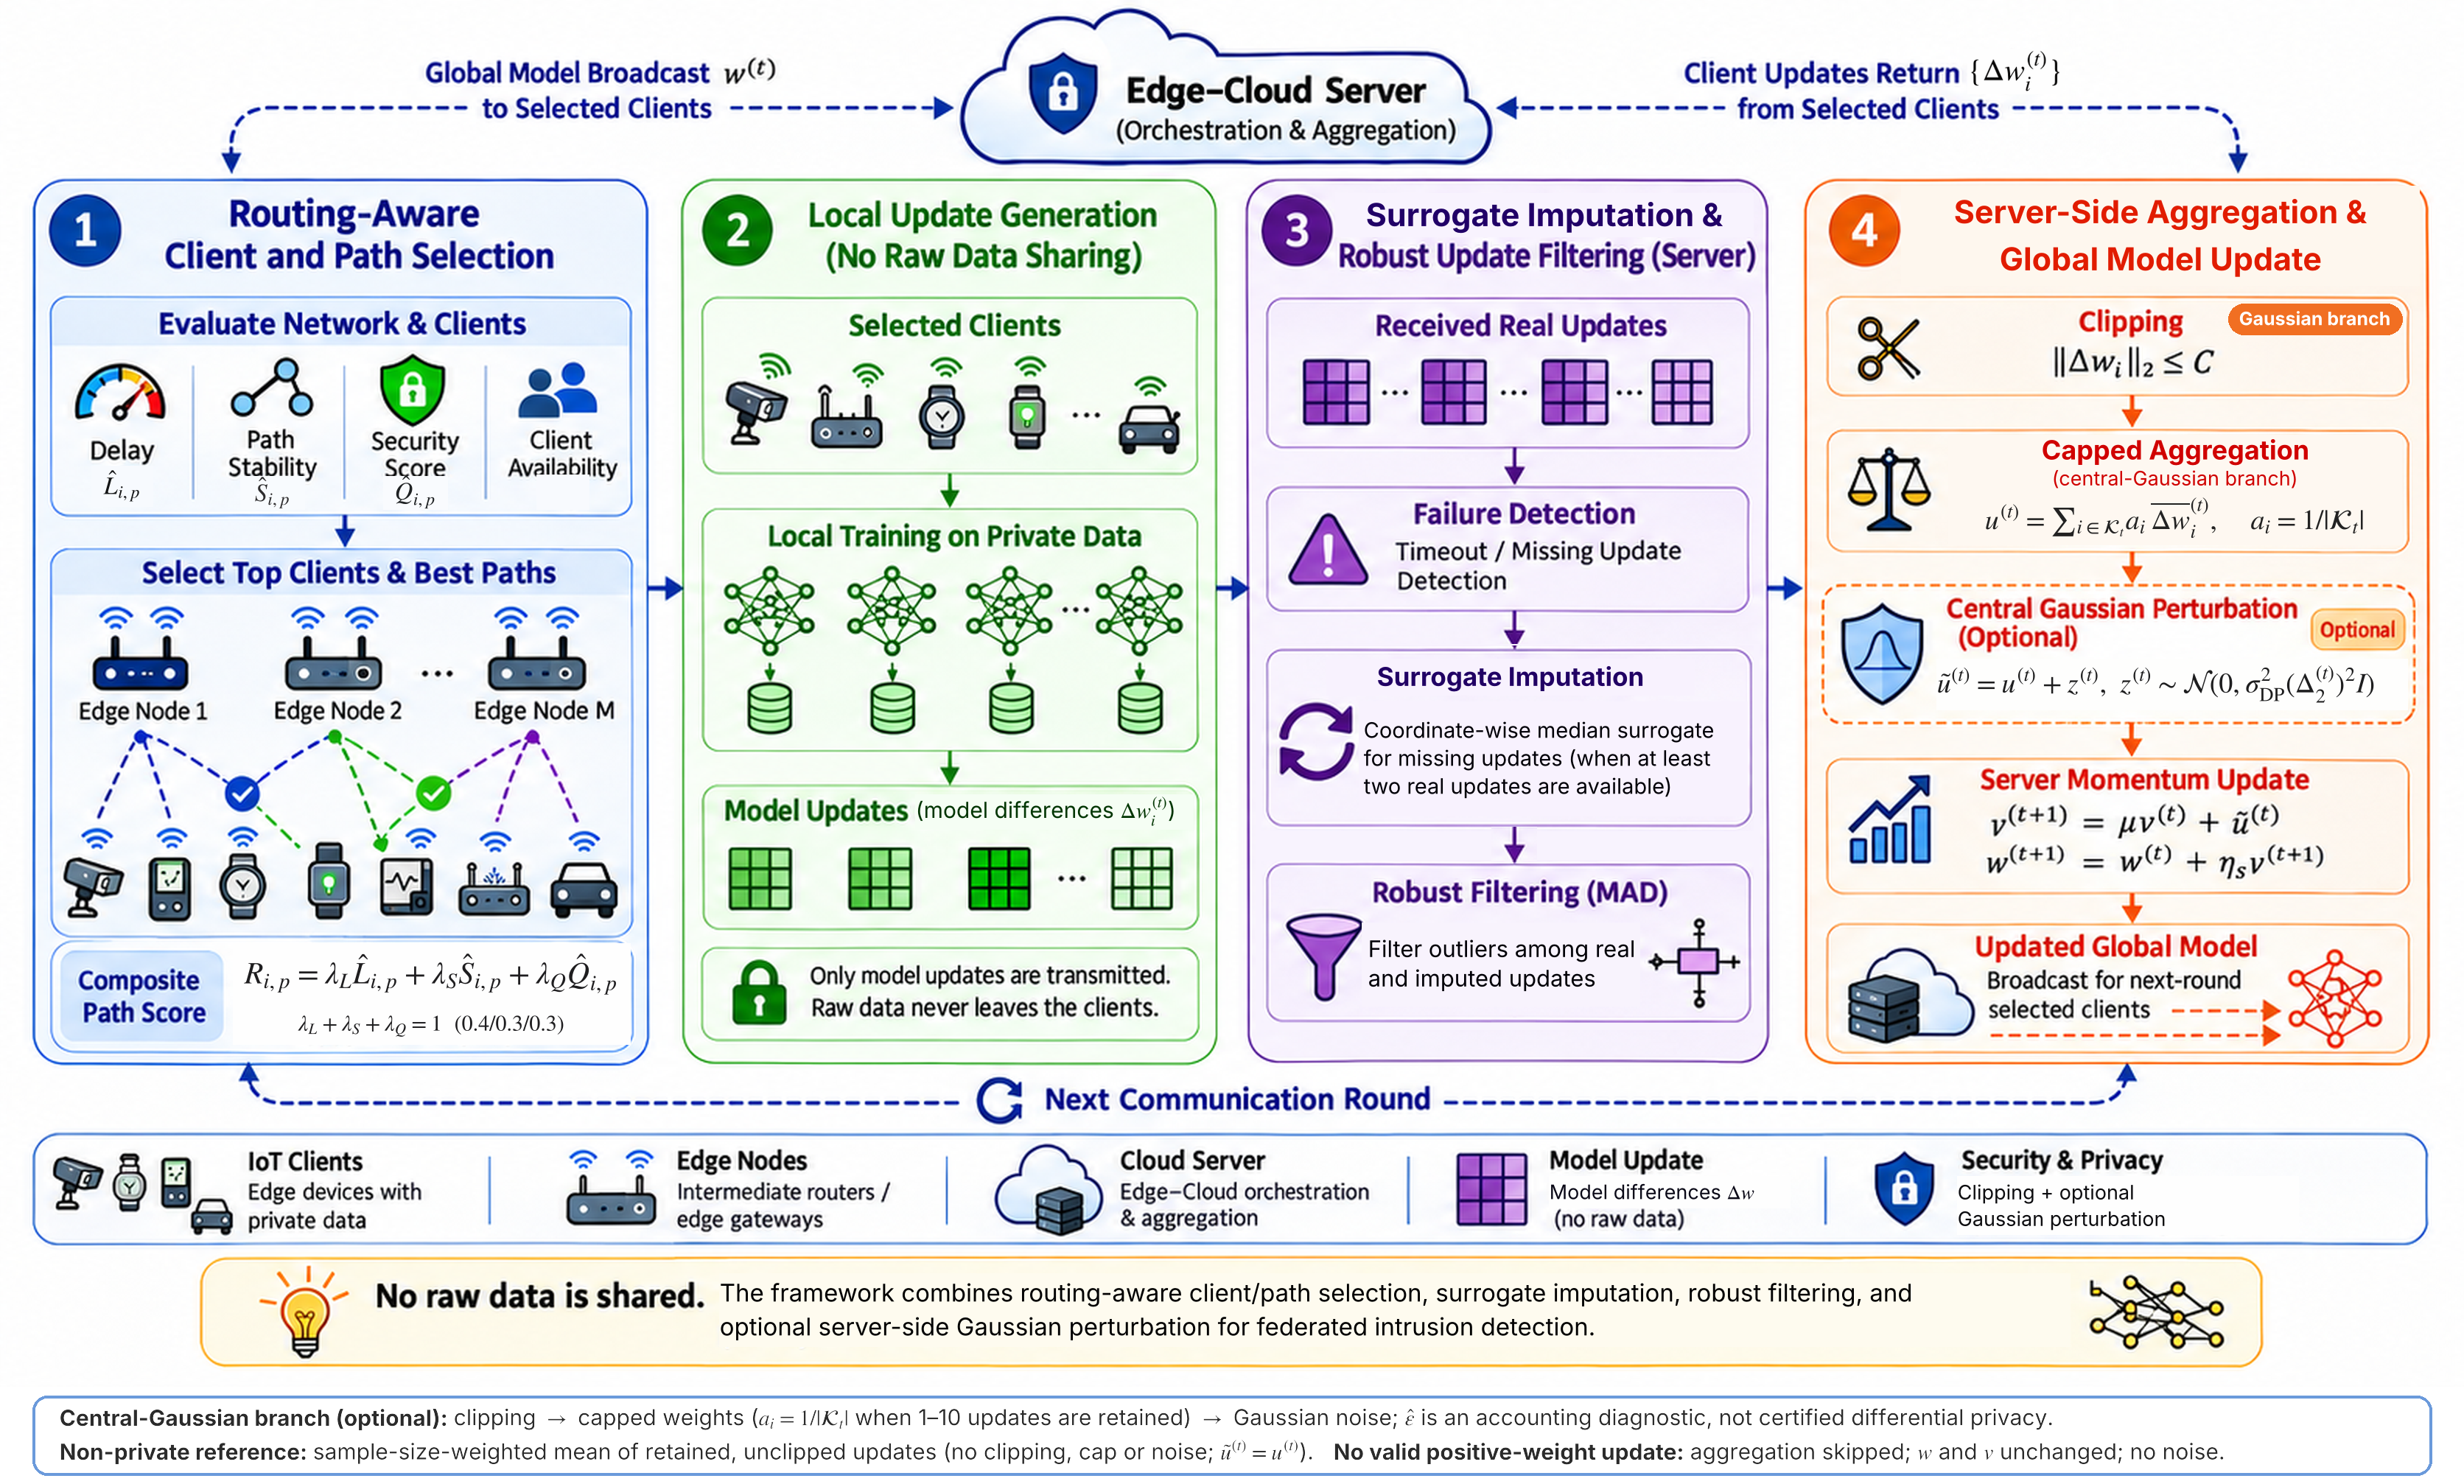
\includegraphics[width=0.93\textwidth]{fig1.png}
	\caption{Routing-aware Edge--Cloud federated IDS architecture.
		In the primary reference configuration, median imputation precedes
		MAD filtering; the real-only filtering control reverses that order.
		Clipping and capped normalization apply only to the central-Gaussian
		branch, not to non-private aggregation.}
	\label{fig:framework-overview}
\end{figure*}
	
	\subsection{Routing-Aware Client and Path Selection}
	\label{subsec:routing-selection}
	
	At the beginning of each communication round, before model updates
	are exchanged, the proposed framework evaluates the communication
	state of the Edge--Cloud network. In IoT environments, the quality of
	the transmission path directly affects end-to-end delay, packet
	delivery ratio, communication stability, and the reliability of the
	federated learning process.
	
	Therefore, the proposed method does not select communication paths
	solely based on link availability. Instead, delay, path stability,
	and path security are jointly considered in the routing decision.
	For each available client \(i\) in communication round \(t\), a set
	of candidate paths \(\mathcal{P}_{i}^{(t)}\) is considered. The
	routing score and the best selected path are defined as
	
	\begin{equation}
		\begin{aligned}
			R_{i,p}^{(t)}
			&=
			\lambda_{L}\widehat{L}_{i,p}^{(t)}
			+
			\lambda_{S}\widehat{S}_{i,p}^{(t)}
			+
			\lambda_{Q}\widehat{Q}_{i,p}^{(t)},\\
			p_{i}^{*(t)}
			&=
			\operatorname*{arg\,max}_{p\in\mathcal{P}_{i}^{(t)}}
			R_{i,p}^{(t)}.
		\end{aligned}
		\label{eq:routing-selection}
	\end{equation}
	
	In Eq.~\eqref{eq:routing-selection},
	\(\widehat{L}_{i,p}^{(t)}\) denotes the normalized delay score,
	where a larger value represents lower delay and better communication
	quality. Similarly, \(\widehat{S}_{i,p}^{(t)}\) and
	\(\widehat{Q}_{i,p}^{(t)}\) denote the normalized path-stability and
	path-security scores, respectively. The non-negative weighting
	coefficients satisfy
	\(\lambda_{L}+\lambda_{S}+\lambda_{Q}=1\).
	
The participating clients are selected according to the best
achievable routing score of each client and the client participation ratio
\(\rho\):
	
	\begin{equation}
		\begin{aligned}
			q_{i}^{(t)}
			&=
			\max_{p\in\mathcal{P}_{i}^{(t)}}
			R_{i,p}^{(t)},\\
			\mathcal{S}_{t}
			&=
			\operatorname{Top}_{\lceil\rho N\rceil}
			\left\{
			q_{i}^{(t)}
			\right\}_{i=1}^{N}.
		\end{aligned}
		\label{eq:client-selection}
	\end{equation}
	
	As shown in Eq.~\eqref{eq:client-selection}, the
	\(\lceil\rho N\rceil\) clients with the highest communication and
	routing scores are selected to participate in round \(t\). This
	design aligns the federated learning process with the current network
	condition and reduces the participation of clients whose available
	paths are weak, unstable, or insecure.
	

The selection strategy intentionally prioritizes communication
reliability. Selecting a fixed number of clients per round does
not guarantee participation coverage or fairness: clients with
persistently weaker routes may be underrepresented. The effects
on participation concentration are examined in
Section~\ref{subsec:attack-routing-tradeoffs}, but worst-client
performance under correlated route quality and local label
distributions remains outside the evaluated scope.
	
	\subsection{Local Update Generation without Raw Data Sharing}
	\label{subsec:local-update}
	
	In each communication round \(t\), every selected IoT client receives
	the current global model from the Edge--Cloud server and performs
	local training using only its private dataset. Raw data are not
	transmitted to the central server, other clients, or the cloud layer.
	This design reduces direct raw-data exposure and communication
	overhead while keeping local data under the control of each IoT
	client.
	
	Let \(\mathcal{D}_{i}\) denote the private dataset of client \(i\),
	containing \(n_i\) local samples. The local learning objective is
	defined by the empirical loss function
	
	\begin{equation}
		\mathcal{L}_{i}(w)
		=
		\frac{1}{n_i}
		\sum_{j=1}^{n_i}
		\ell\left(f(x_{ij};w),y_{ij}\right).
		\label{eq:local-loss}
	\end{equation}
	
	In Eq.~\eqref{eq:local-loss}, \(\mathcal{L}_{i}(w)\) denotes the
	empirical loss over the private dataset of client \(i\);
	\(x_{ij}\) and \(y_{ij}\) represent the input and label of local
	sample \(j\), respectively; \(f(\cdot;w)\) is the local prediction
	model; and \(\ell(\cdot)\) is the loss function.
	
	Starting from the current global model \(w^{(t)}\), client \(i\)
	performs \(E\) local epochs using learning rate \(\eta\). The local
	optimization process and the resulting model update are defined
	jointly as
	
	\begin{equation}
		\begin{aligned}
			w_{i}^{(t,E)}
			&=
			\operatorname{LocalOpt}
			\left(
			w^{(t)},\mathcal{D}_{i},E,\eta
			\right),\\
			\Delta w_{i}^{(t)}
			&=
			w_{i}^{(t,E)}-w^{(t)}.
		\end{aligned}
		\label{eq:local-training-update}
	\end{equation}
	
	As expressed in Eq.~\eqref{eq:local-training-update}, local training
	starts from the global model received at the beginning of round
	\(t\). After \(E\) local epochs, client \(i\) obtains the trained
	local model \(w_{i}^{(t,E)}\).
	
	Instead of transmitting raw data or the complete local dataset, the
	client sends only the model difference
	\(\Delta w_{i}^{(t)}\) through the selected communication path
	\(p_{i}^{*(t)}\). The Edge--Cloud server subsequently processes the
	received updates using failure recovery, robust filtering, and
	privacy-aware aggregation.
	\subsection{Surrogate Imputation and Robust Update Filtering}
	\label{subsec:failure-recovery}
	
	In practical Edge--Cloud IoT environments, some selected clients may
	fail to deliver their updates during a communication round. Client
	failures, link outages, excessive path delay, network congestion, or
	adversarial behavior may cause updates to arrive late, be lost, or
	deviate substantially from the main update direction.
	
	Before aggregation, the Edge--Cloud server identifies the successfully
	received real updates, denoted by \(\mathcal{U}_{t}\). Two processing
	orders are considered. In the original reference configuration,
	missing-update surrogates are inserted before MAD filtering.
	In the real-only filtering variant, MAD is first applied to received
	real updates, then surrogates are computed from the retained updates.
	
	For the original reference configuration, when a selected client
	fails to deliver its update and \(|\mathcal{U}_{t}|\geq 2\),
	a surrogate update is computed as the coordinate-wise median:
	
\begin{equation}
	\Delta w_{i,\mathrm{rec}}^{(t)}
	=
	\operatorname{Median}_{\mathrm{coord}}
	\left(
	\left\{
	\Delta w_{j}^{(t)}
	\mid j\in\mathcal{U}_{t}
	\right\}
	\right),
	\qquad
	|\mathcal{U}_{t}|\geq 2.
	\label{eq:recovered-update}
\end{equation}
	
	
	The surrogate for each missing update is assigned a reduced raw-weight
	factor \(\chi_{\mathrm{rec}}\). In the non-Gaussian reference,
	this factor affects normalized sample-size weights but does not
	bound the collective surrogate share. In the central-Gaussian branch,
	the implemented cap produces equal applied weights when at most ten
	updates survive (Section~\ref{subsec:private-aggregation}); hence
	\(\chi_{\mathrm{rec}}\) does not down-weight surrogates there.
	Matched imputation-omission comparisons did not establish a detection
	benefit (Section~\ref{subsec:routing-surrogate}).
	
	
	
	The surrogate in Eq.~\eqref{eq:recovered-update} substitutes a
	median direction; it does not recover the missing client's local
	information. With fewer than two received updates the unavailable
	client is excluded. With no received update, aggregation, Gaussian
	noise and accounting are skipped, and the global model is unchanged.
	This zero-update case did not occur in the 40 controlled runs.
	
	After imputation, the server constructs the available update set
	\(\mathcal{V}_{t}\), containing both received real updates and
	imputed surrogate updates. The robust center and the deviation
	of each available update from this center are defined jointly as
	
	\begin{equation}
		\begin{aligned}
			m^{(t)}
			&=
			\operatorname{Median}_{\mathrm{coord}}
			\left(
			\left\{
			\Delta w_{i}^{(t)}
			\mid i\in\mathcal{V}_{t}
			\right\}
			\right),\\
			d_{i}^{(t)}
			&=
			\left\|
			\Delta w_{i}^{(t)}-m^{(t)}
			\right\|_{2},
			\qquad i\in\mathcal{V}_{t}.
		\end{aligned}
		\label{eq:robust-center-deviation}
	\end{equation}
	
	In Eq.~\eqref{eq:robust-center-deviation}, \(m^{(t)}\) represents
	the robust central direction of the available updates, while
	\(d_i^{(t)}\) measures the deviation of update \(i\) from this
	center. Large deviations may result from communication failures,
	highly non-IID data, poisoning attacks, or Byzantine behavior.
	
	For compact notation, define
	\(\mathbf{d}^{(t)}=\{d_i^{(t)}\}_{i\in\mathcal{V}_{t}}\).
	The MAD-based threshold and the resulting reliable update set are
	then defined as
	
	\begin{equation}
		\begin{aligned}
			\tau_{t}
			&=
			\operatorname{Median}\!\left(\mathbf{d}^{(t)}\right)
			+
			1.4826\,k\,
			\operatorname{MAD}\!\left(\mathbf{d}^{(t)}\right),\\
			\mathcal{K}_{t}
			&=
			\left\{
			i\in\mathcal{V}_{t}
			\mid
			d_{i}^{(t)}\leq\tau_{t}
			\right\}.
		\end{aligned}
		\label{eq:mad-reliable-set}
	\end{equation}
	
	Here, \(\operatorname{MAD}(\mathbf{d})=\operatorname{Median}_i
	|d_i-\operatorname{Median}(\mathbf{d})|\). The implementation
	uses a numerical floor of \(10^{-12}\) inside the scaled-MAD term
	to avoid a zero-width threshold. Updates with deviation no greater
	than \(\tau_t\) are retained, and \(k\) sets filtering strictness.
	
	
	The filtering decision applies only to the current communication
	round and should not be interpreted as a permanent malicious-client
	label. A large deviation may also be caused by legitimate statistical
	heterogeneity.
	
	If \(\mathcal{K}_{t}\) becomes empty, the update closest to the robust
	center is retained as a fallback. In other words, the client with
	\(i^{*}=\operatorname*{arg\,min}_{i\in\mathcal{V}_{t}}d_i^{(t)}\)
	is retained to prevent interruption of the current aggregation round.
	
	\subsection{Privacy-Aware Aggregation and Global Model Update}
	\label{subsec:private-aggregation}
	
Following robust filtering and any configured surrogate imputation,
	the Edge--Cloud server constructs the aggregate from the retained
	updates. In the central-Gaussian branch the retained updates are
clipped and aggregated with capped weights before noise is added;
in the non-private reference the retained updates are instead
aggregated without this clipping or cap. Server momentum acts
on whichever aggregate the configured branch supplies.
	
	In the central-Gaussian branch only, each reliable update is
clipped using threshold \(C\):
	
	\begin{equation}
		\overline{\Delta w}_{i}^{(t)}
		=
		\Delta w_{i}^{(t)}
		\min\left(
		1,
		\frac{C}
		{\left\|\Delta w_{i}^{(t)}\right\|_{2}+\xi}
		\right),
		\qquad i\in\mathcal{K}_{t},
		\label{eq:update-clipping}
	\end{equation}
	
	where \(\xi>0\) is a small constant that prevents division by zero.
	Consequently,
	\(\|\overline{\Delta w}_{i}^{(t)}\|_{2}\leq C\).
Clipping limits the influence of unusually large client updates and
controls the update magnitude used in the subsequent aggregation and
noise-calibration procedure.
	
Before normalization, each received real update has a raw weight
\(b_i^{(t)}\) proportional to its client sample size; a surrogate's
raw weight is further multiplied by \(\chi_{\mathrm{rec}}\).
In the non-private branch, weights are normalized without a cap:
\(a_i^{(t)}=b_i^{(t)}/\sum_{j\in\mathcal K_t}b_j^{(t)}\),
provided the sum is positive. Only the central-Gaussian branch uses
the feasible cap and \(\operatorname{CapNormalize}\) shown below. In
the Gaussian branch the aggregate uses clipped updates; the
non-private reference aggregates retained, unclipped updates.


\begin{equation}
	\begin{aligned}
		\overline{a}_{\max}^{(t)}
		&=
		\max\left(
		a_{\max},
		\frac{1}{|\mathcal{K}_{t}|}
		\right),\\
		\left\{a_i^{(t)}\right\}_{i\in\mathcal{K}_{t}}
		&=
		\operatorname{CapNormalize}
		\left(
		\left\{b_i^{(t)}\right\}_{i\in\mathcal{K}_{t}},
		\overline{a}_{\max}^{(t)}
		\right),\\
		u^{(t)}
		&=
		\sum_{i\in\mathcal{K}_{t}}
		a_i^{(t)}
		\overline{\Delta w}_{i}^{(t)}.
	\end{aligned}
	\label{eq:capped-weighting}
\end{equation}
	Operationally, $\operatorname{CapNormalize}$ repeatedly normalizes
	the raw weights of active entries to the remaining unit mass,
	fixes entries whose tentative share exceeds the feasible cap at
	that cap, and redistributes the residual mass. If all remaining
	active raw weights are zero after some entries have been capped,
	residual mass is divided equally among those active entries.
	The complete zero-sum input is handled separately by abstention
	before normalization. With positive total raw weight, the
	resulting weights sum to one and satisfy
	$0\leq a_i^{(t)}\leq\overline a_{\max}^{(t)}$.
For a round with a positive raw-weight sum, the central-Gaussian
weights satisfy \(\sum_{i\in\mathcal K_t}a_i^{(t)}=1\) and
\(0\leq a_i^{(t)}\leq\overline a_{\max}^{(t)}\).
With \(a_{\max}=0.1\) and at most ten retained updates,
\(\overline a_{\max}^{(t)}=1/|\mathcal K_t|\). Because the
weights sum to one, every retained update then receives exactly
\(a_i^{(t)}=1/|\mathcal K_t|\), regardless of client size or
\(\chi_{\mathrm{rec}}\). A weight audit found uniform applied
weights for all 2,750 central-Gaussian aggregation rounds with at
most ten retained updates (maximum deviation \(1.4\times10^{-16}\));
the remaining audited rounds included larger client sets or abstentions.
In the original proposed configurations (300 rounds), fewer than
ten updates survived in 92\% of rounds (minimum six), yielding
a largest applied share of 0.167. Surrogates jointly carried a mean
weight share of 0.30 (maximum 1.0), and only surrogates remained
in ten rounds. Thus the Gaussian-path cap does not implement
surrogate down-weighting and is not evidence of an independent
weighting benefit.

When all retained raw weights sum to zero, the SUPP\_V2
implementation takes a \emph{no-valid-contribution} abstention:
the global model and server momentum remain unchanged, and no
Gaussian noise is released. Release-based and attempted-round
accounting diagnostics are recorded separately. The abstention
branch does not alter rounds with a positive raw-weight sum; in
such rounds, the feasible cap gives every retained update weight
$1/|\mathcal K_t|$ when at most ten updates remain, even if a
surrogate's raw weight was zero.


	For noise calibration, the implementation uses the following
	effective \(L_2\)-sensitivity scale for the clipped weighted aggregate:
	
	\begin{equation}
		\Delta_{2}^{(t)}
		=
		\varphi C
		\max_{i\in\mathcal{K}_{t}}
		a_i^{(t)}.
		\label{eq:aggregate-sensitivity}
	\end{equation}
	
The coefficient \(\varphi\) is the adjacency-scaling factor used by
the implementation. The experiments use \(\varphi=1\), corresponding
to the remove/add configuration, while \(\varphi=2\) can be used for
a more conservative replace-one scaling. Because the retained client
set and the capped normalized weights are data-dependent,
\(\Delta_{2}^{(t)}\) is used here as an effective noise-calibration
scale rather than claimed as a formal global sensitivity bound for
the complete routing, filtering, and aggregation pipeline.
	
When the server-side Gaussian privacy mode is enabled, the
weighted aggregate is perturbed as follows:
	
	\begin{equation}
		\begin{aligned}
			\widetilde{u}^{(t)}
			&=
			u^{(t)}+z^{(t)},\\
			z^{(t)}
			&\sim
			\mathcal{N}\left(
			0,
			\sigma_{\mathrm{DP}}^{2}
			\left(\Delta_{2}^{(t)}\right)^{2}I
			\right).
		\end{aligned}
		\label{eq:gaussian-mechanism}
	\end{equation}
	
	Here, \(\sigma_{\mathrm{DP}}\) is the Gaussian noise multiplier and
	\(I\) denotes the identity matrix. Because the Gaussian noise is added
	by the server after filtering, clipping, and weighted aggregation, the
	mechanism follows a server-side central Gaussian perturbation design
	and is evaluated using the estimated central-DP accounting procedure
	described below.
	
The implementation computes a diagnostic RDP-based estimate using
an internal approximation to the Poisson-subsampled Gaussian
mechanism and integer Renyi orders $\alpha=2,\ldots,128$.
The scaling factor $\varphi=1$ follows the implemented add/remove
noise-calibration convention. This is not a proof of record-level
or client-level differential privacy: actual participant selection,
filtering, and weighting do not satisfy the assumptions needed
for an end-to-end certified adjacency-based privacy bound. For accounting, the routing-aware top-\(k\)
participation fraction is represented by
\(q=|\mathcal{S}_t|/N=0.2\) and treated as a Poisson-sampling
approximation. The noise multiplier is calibrated to the target budget. Because the actual routing-aware selection is
deterministic rather than Poisson and the robust filtering stage is
data-dependent, the resulting \(\widehat{\varepsilon}\) is reported
as an estimated central-DP budget under a trusted or semi-trusted
server assumption, not as a formal end-to-end guarantee.
The aggregation server receives individual client model updates
before server-side perturbation. Consequently, Gaussian noise
added after aggregation does not protect these updates from the
receiving server. The study does not establish record-level or
client-level differential privacy for the released model under
the actual adaptive selection and filtering mechanism.

	Finally, server momentum and the global-model update are performed
	jointly as
	
	\begin{equation}
		\begin{aligned}
			v^{(t+1)}
			&=
			\mu v^{(t)}
			+
			\widetilde{u}^{(t)},\\
			w^{(t+1)}
			&=
			w^{(t)}
			+
			\eta_s v^{(t+1)}.
		\end{aligned}
		\label{eq:global-update}
	\end{equation}
	
	In Eq.~\eqref{eq:global-update}, \(\mu\) is the server momentum
	coefficient and \(\eta_s\) is the server learning rate.
	Server momentum accumulates the current aggregate with the
	previous server velocity. Its effect on training stability
	depends on the evaluated configuration and is not assumed
	to improve every outcome.
	The updated global model \(w^{(t+1)}\) is then distributed to the
	clients selected for the next communication round. The complete
	procedure is summarized in Table~\ref{alg:proposed-framework}.
	
\begin{table*}[!t]
		\setlength{\abovecaptionskip}{2pt}
	\setlength{\belowcaptionskip}{2pt}
	\caption{Pseudocode of the proposed routing-aware, privacy-aware,
		and fault-tolerant federated learning framework.}
	\label{alg:proposed-framework}
	\centering
	\scriptsize
	\setlength{\tabcolsep}{4.5pt}
	\renewcommand{\arraystretch}{0.94}
	
	\begin{tabularx}{0.96\textwidth}{
			@{}
			>{\centering\arraybackslash}p{0.045\textwidth}
			>{\raggedright\arraybackslash}X
			@{}}
		\toprule
		
		\multicolumn{2}{@{}l}{
			\textbf{Input:}
			Local datasets \(\{\mathcal{D}_i\}_{i=1}^{N}\);
			initial model \(w^{(0)}\);
			\(T,E,\eta,\eta_s,\mu,\rho,\lambda_L,\lambda_S,\lambda_Q,
		C,\varepsilon,\delta,k,a_{\max},
			\chi_{\mathrm{rec}},\xi\).
		} \\
		
		\multicolumn{2}{@{}l}{
			\textbf{Output:}
			Final global model \(w^{(T)}\) and IDS, routing, privacy,
			and resilience metrics.
		} \\
		
		\midrule
		
		1 &
	Initialize \(v^{(0)}=0\) and calibrate
	\(\sigma_{\mathrm{DP}}\) for the target
	\((\varepsilon,\delta)\).\\
		2 &
		\pkw{for} \(t=0,\ldots,T-1\) \pkw{do} \\
		
		3 &
		\pindent
		Update the Edge--Cloud network state and compute candidate paths. \\
		
		4 &
		\pindent
		Compute routing scores using latency, stability, and security;
		select \(\mathcal{S}_t\) and assign \(p_i^{*(t)}\). \\
		
		5 &
		\pindent
		Broadcast \(w^{(t)}\) to the selected clients. \\
		
		6 &
		\pindent
		\pkw{for each} \(i\in\mathcal{S}_t\)
		\pkw{in parallel do} \\
		
		7 &
		\pindenttwo
		Train on \(\mathcal{D}_i\) for \(E\) local epochs and compute
		\(\Delta w_i^{(t)}=w_i^{(t,E)}-w^{(t)}\). \\
		
		8 &
		\pindenttwo
		Transmit \(\Delta w_i^{(t)}\) through
		\(p_i^{*(t)}\). \\
		
		9 &
		\pindent
		\pkw{end for} \\
		
		10 &
		\pindent
If no update arrived, keep \(w^{(t)}\) and \(v^{(t)}\) unchanged, skip aggregation/noise/accounting, and continue; otherwise detect missing updates. \\

		
		11 &
		\pindent
		\pkw{if} failures exist and
		\(|\mathcal{U}_t|\geq2\) \pkw{then} \\
		
		12 &
		\pindenttwo
		Insert coordinate-wise median surrogates for missing updates
		and assign raw-weight factor \(\chi_{\mathrm{rec}}\). \\
		
		13 &
		\pindent
		\pkw{else} \\
		
		14 &
		\pindenttwo
		Exclude unavailable clients from the current aggregation round. \\
		
		15 &
		\pindent
		\pkw{end if} \\
		
		16 &
		\pindent
		Construct \(\mathcal{V}_t\), compute the robust center and
		MAD-based threshold, and obtain the reliable set
		\(\mathcal{K}_t\). \\
		
		17 &
		\pindent
		If retained raw weights sum to zero, abstain with unchanged model and
momentum. Otherwise, in central-Gaussian mode clip and cap-normalize;
in non-private mode aggregate retained un-clipped updates. \\\
		
		18 &
		\pindent
		For the Gaussian branch compute the clipped aggregate and noise
calibration scale; otherwise compute the un-clipped aggregate. \\\
		
		
		19 &
		\pindent
		In a non-abstaining Gaussian round, add noise and count one noisy
		release; otherwise use \(\widetilde{u}^{(t)}=u^{(t)}\). Report
		attempted and released privacy rounds separately. \\
		
		20 &
		\pindent
		Update
		\(v^{(t+1)}=\mu v^{(t)}+\widetilde{u}^{(t)}\) and
		\(w^{(t+1)}=w^{(t)}+\eta_s v^{(t+1)}\). \\
		
		21 &
		\pindent
		Compute and log IDS, routing, privacy, and resilience metrics. \\
		
		22 &
		\pkw{end for} \\
		
		23 &
		\pkw{return} \(w^{(T)}\). \\
		
		\bottomrule
	\end{tabularx}
\end{table*}

	\section{Simulation}
	\label{sec:experiments}
	
	The proposed framework was evaluated in a simulated Edge--Cloud
	federated learning environment using CICIoT2023 and UNSW-NB15.
	The evaluation considers intrusion-detection performance, routing
	reliability, client participation, attack robustness, failure
	recovery, and privacy-related behavior. The controlled comparisons include FedAvg under distinct
	client-selection and path-assignment policies, a non-private
	MAD-filtered reference, and a Gaussian-perturbed FedAvg control.
	The modular and hierarchical FL architectures discussed in
	\cite{almeida2025modular,chen2025hierarchical} were not
	re-implemented as experimental baselines.
	
	CICIoT2023 serves as the primary IoT-oriented benchmark, while
	UNSW-NB15 provides a complementary network-intrusion benchmark
	with different traffic characteristics. Component-wise comparisons
	are used to distinguish the effects of client selection, delivery
	behavior, robust filtering, surrogate imputation, weighting, and
	server momentum.
	
	\subsection{Experimental Setup and Simulation Settings}
	\label{subsec:experimental-setup}
	
	An Edge--Cloud-based federated learning environment was simulated to
	evaluate the proposed framework. In this environment, IoT clients do
	not transmit raw data to the server. Instead, only locally generated
	model updates are transmitted through the selected communication
	paths.
	

After receiving client updates, the Edge--Cloud server performs
failure detection, median-based surrogate imputation where possible,
robust filtering and a configuration-dependent aggregation branch.
Only the central-Gaussian branch clips, caps and perturbs retained
updates before the momentum-based model
update; the order of filtering and imputation is configuration-specific.
	
	Two network-intrusion datasets were used in the experiments.
	CICIoT2023 was selected as the primary dataset because it contains
	diverse IoT traffic and multiple attack patterns and is therefore
	closely aligned with the Edge--Cloud IoT scenario considered in this
	study.
	
	For CICIoT2023, the label of each sample was extracted from its
	corresponding folder or attack category. The intrusion detection task
	was formulated as a binary classification problem consisting of
	attack and benign traffic.
	
	
	The locked CICIoT2023 preparation contains 926,133 training and
	146,626 validation records with 39 numerical features; the reserved
	300,000-record test partition was not accessed. Preparation removed
	73,867 feature-identical training duplicates and 53,374 validation
	duplicates. The \texttt{file\_group} policy separated source-file
	groups for 17 of 34 classes with enough files; the remaining 17
	classes were row-stratified. Thus, this is not a universal
	capture-disjoint or held-out-device evaluation. The validation pool
	was divided into distinct calibration, checkpoint-selection, and
	report partitions, with 1,564 benign records in each report partition.
	
	UNSW-NB15 is a separate within-dataset benchmark rather than a
	cross-dataset transfer experiment. Its 175,341 official training
	records were divided into 150,293 training records and a 25,048-record
	validation pool. For seed 12, the calibration, selection, and report
	partitions contain 8,350, 8,350, and 8,348 records, respectively
	(other seeds differ by at most four records). The 82,332-record
	official test partition was not accessed. Its 42 raw features become
194 numeric features after categorical encoding. The split and preparation fingerprints are documented in the locked
	manifests. Categorical encoders and numerical scalers are fitted
	only on the training portion; validation records are transformed
	without refitting. Non-IID client partitions use a class-conditional
	Dirichlet allocation with $\alpha_{\mathrm{Dir}}=0.5$ across 50
	clients, followed by rebalancing when needed to enforce at least
	100 training records per client.
	

\paragraph{Network model}
Each client has three candidate paths, one through each edge node.
Initial client--edge links use uniformly drawn latency (5--80~ms),
stability (0.75--0.99), security (0.60--0.98), and bandwidth
(20--150~Mbit/s); corresponding edge--cloud ranges are 5--50~ms,
0.85--0.995, 0.75--0.99, and 100--1000~Mbit/s. Link states persist across rounds and evolve through multiplicative
Gaussian latency perturbations and additive Gaussian stability and
security perturbations (dynamic scale $\sigma=0.025$). This creates
temporally correlated link attributes. Each client--edge link has a
per-round outage draw with probability 0.01; an outage reduces its
simulated stability to at most 0.05 rather than automatically
removing an update. Separately, a selected client may fail under
an independent explicit-failure draw ($p_f=0.1$). A real update is
unavailable when that explicit failure occurs or when the simulated
network transfer is not delivered. Path delay sums link delays, stability multiplies
link stabilities, and security takes the minimum. Routing scores use
per-client min--max-normalized latency, stability, and security with
weights 0.4/0.3/0.3 and the simulator's current, directly accessible
link state. Security is a simulated link attribute, not measured
attack detection. Packet delivery uses 100 independent packet
attempts per update; update arrival is a separate Bernoulli draw.
Transmission delay adds serialization and stochastic jitter to path
latency. Queueing, congestion and physical measurement error are not
modeled. The reference delivery model has no retransmissions;
separate packet-coupled controls model retransmission attempts,
and account for their simulated time and link-byte overhead.

\paragraph{Attack model}
In the evaluated sign-flip scenario, an attack replaces the update
of a malicious client with $-5\Delta w_i^{(t)}$. Exactly two of ten
selected clients are assigned as malicious in each round,
independently of network state. Adaptive poisoning, collusion, and
security-score manipulation were not evaluated.

The same multilayer perceptron (MLP) architecture was used across
matched configurations wherever applicable. The network has three
hidden layers with 128, 96 and 64 units, respectively, ReLU
activations, dropout of 0.2 after the last hidden layer, and a
two-logit output layer for binary classification. Local models
were trained using the Adam optimizer and cross-entropy loss,
with a learning rate of $3\times10^{-4}$, batch size of 256,
two local epochs and zero weight decay. The controlled
ablation comparisons use five paired random seeds (12--16).
Checkpoint selection, decision-threshold calibration, and metric
reporting are kept separate within the validation-based evaluation
protocol. The reserved test partitions were not accessed during
these reported controlled comparisons and ablation runs.
Results distinguish selected-checkpoint and final-round
performance, and error bars indicate one standard deviation
across the five seeds.

	
	\subsection{Evaluation Metrics}
	\label{subsec:evaluation-metrics}
	
	To provide a comprehensive evaluation of the proposed framework,
	the evaluation metrics were grouped into four categories:
	intrusion-detection metrics, network-performance metrics,
	resilience metrics, and privacy and communication-cost metrics.
	
	Intrusion-detection performance was evaluated using Accuracy,
	Precision, Recall, F1-score, ROC-AUC, PR-AUC, and the false
	positive rate (FPR). In all classification metrics, attack traffic
	was considered the positive class, whereas benign traffic was
	considered the negative class.
	
The standard binary-classification metrics are defined below.
Here, \(TP\), \(TN\), \(FP\), and \(FN\) denote true positives,
true negatives, false positives, and false negatives,
respectively. Accuracy measures overall classification
correctness, while Precision and Recall characterize
attack detection performance.

\begin{equation}
	\mathrm{Accuracy}
	=
	\frac{TP+TN}
	{TP+TN+FP+FN},
	\label{eq:accuracy}
\end{equation}

\begin{equation}
	\mathrm{Precision}
	=
	\frac{TP}{TP+FP}.
	\label{eq:precision}
\end{equation}

\begin{equation}
	\mathrm{Recall}
	=
	\frac{TP}{TP+FN}.
	\label{eq:recall}
\end{equation}

The F1-score is the harmonic mean of Precision and Recall.
ROC-AUC measures discrimination across classification
thresholds, whereas PR-AUC summarizes the precision--recall
trade-off and is informative under class imbalance.

\begin{equation}
	\mathrm{F1\mbox{-}score}
	=
	\frac{
		2\,\mathrm{Precision}\,\mathrm{Recall}
	}{
		\mathrm{Precision}+\mathrm{Recall}
	}.
	\label{eq:f1-score}
\end{equation}

\begin{equation}
	\mathrm{ROC\mbox{-}AUC}
	=
	\int_{0}^{1}
	\mathrm{TPR}(\mathrm{FPR})
	\,d(\mathrm{FPR}),
	\label{eq:roc-auc}
\end{equation}

\begin{equation}
	\mathrm{PR\mbox{-}AUC}
	=
	\int_{0}^{1}
	\mathrm{Precision}(\mathrm{Recall})
	\,d(\mathrm{Recall}).
	\label{eq:pr-auc}
\end{equation}

Here, \(\mathrm{TPR}\) is the true positive rate and is
equivalent to Recall. The false positive rate measures
the proportion of benign samples incorrectly classified
as attacks:

\begin{equation}
	\mathrm{FPR}
	=
	\frac{FP}{FP+TN}.
	\label{eq:fpr}
\end{equation}
	
	
	A lower FPR indicates fewer false security alerts. The operating
	threshold is selected on the calibration partition from 1,001
	candidates satisfying FPR $\leq0.15$ and recall $\geq0.60$,
	maximizing recall (ties: F1, balanced accuracy, closeness to 0.5).
	If no candidate is feasible, recall is maximized subject to the
	FPR cap, with infeasibility flagged. The observed FPR near 0.15
	is consequently cap-driven, not operationally low. Checkpoints
	are selected by selection-partition ROC--AUC with minimum
	improvement $10^{-4}$. Network metrics include delivery delay,
	packet PDR, path stability, and transfer efficiency.
	
	End-to-end delay measures the average time required for a packet or
	model update to travel from its source to the destination. It is
	calculated as
	
	\begin{equation}
		\mathrm{E2E\mbox{-}Delay}
		=
		\frac{1}{M}
		\sum_{m=1}^{M}
		\left(
		t_{m}^{\mathrm{received}}
		-
		t_{m}^{\mathrm{sent}}
		\right),
		\label{eq:e2e-delay}
	\end{equation}
	
	where \(M\) is the number of successfully delivered packets or model
	updates, while \(t_{m}^{\mathrm{sent}}\) and
	\(t_{m}^{\mathrm{received}}\) denote the transmission and reception
	times of packet or update \(m\), respectively. A lower end-to-end
	delay indicates faster update transmission and more efficient
	routing.
	

First-transmission packet delivery ratio (PDR) measures the fraction
of attempted packets successfully received on their initial
transmission. It is distinct from the final successful delivery
of a model update:

	
	\begin{equation}
		\mathrm{PDR}
		=
		\frac{N_{\mathrm{received}}}
		{N_{\mathrm{sent}}},
		\label{eq:pdr}
	\end{equation}
	
	where \(N_{\mathrm{received}}\) and \(N_{\mathrm{sent}}\) denote the
	numbers of successfully received and transmitted packets,
	respectively. A higher PDR indicates more reliable communication and
	better link quality.
	
	
	The reported path-stability score averages the simulated link
	stability and round-to-round route persistence of selected paths:
	
	\begin{equation}
		\mathrm{Path\ Stability}
		=\frac{1}{|\mathcal{S}|}\sum_{(i,t)\in\mathcal{S}}
		\bigl(0.5s_i^{(t)}+0.5\varrho_i^{(t)}\bigr),
		\label{eq:path-stability}
	\end{equation}
	
	where \(\mathcal{S}\) indexes evaluated selected paths,
	\(s_i^{(t)}\) is their link-stability value, and
	\(\varrho_i^{(t)}=1\) when the client retains its previous
	edge node (zero otherwise). The score is not simply the
	fraction of paths above a binary stability threshold.
	
	
	Transfer efficiency measures the amount of successfully delivered
	data or model updates relative to the end-to-end transmission time:
	
	\begin{equation}
		\mathrm{Transfer\ Efficiency}
		=
		\frac{D_{\mathrm{delivered}}}
		{T_{\mathrm{E2E}}},
		\label{eq:transfer-efficiency}
	\end{equation}
	
	where \(D_{\mathrm{delivered}}\) represents the successfully delivered
	data or model-update volume and \(T_{\mathrm{E2E}}\) denotes the
	corresponding end-to-end transmission time. A higher transfer
	efficiency indicates more effective use of the available network
	resources.
	Resilience was evaluated using the F1 recovery fraction, recovery
	rounds, and surrogate-imputation coverage. Privacy and communication behavior was evaluated
	using the estimated privacy budget, noise-to-signal ratio, and
	communication cost.
	

	
The estimated privacy budget is tracked using an RDP accountant based
on the accounting participation fraction, the number of
privacy-releasing rounds, the calibrated Gaussian noise multiplier,
and the DP failure probability:
	
\begin{equation}
	\widehat{\varepsilon}
	=
	\operatorname{RDPAccountant}
	\left(
	q,R_{\mathrm{DP}},\sigma_{\mathrm{DP}},\delta
	\right).
	\label{eq:estimated-privacy}
\end{equation}
	
	In Eq.~\eqref{eq:estimated-privacy},
	\(q=|\mathcal{S}_t|/N=0.2\) is the participation fraction used as a
	Poisson-sampling approximation, \(R_{\mathrm{DP}}\leq T\) is the
	number of rounds that actually release a noisy aggregate,
	\(\sigma_{\mathrm{DP}}\) is the calibrated Gaussian noise multiplier,
	and \(\delta\) is the DP failure probability.
	Accordingly, the reported \(\widehat{\varepsilon}\) is an accounting
	estimate rather than a formal guarantee for the deterministic
	routing-aware client selection and data-dependent filtering pipeline.
	
	The noise-to-signal ratio (NSR) measures the magnitude of the injected
	privacy noise relative to the magnitude of the aggregated update:
	
	\begin{equation}
		\mathrm{NSR}^{(t)}
		=
		\frac{
			\left\|z^{(t)}\right\|_{2}
		}{
			\left\|u^{(t)}\right\|_{2}+\xi
		}.
		\label{eq:nsr}
	\end{equation}
	
	Here, \(z^{(t)}\) denotes the Gaussian noise injected during round
	\(t\), \(u^{(t)}\) is the aggregated update before noise addition, and
	\(\xi>0\) prevents division by zero. A lower NSR indicates that the
	privacy noise has a smaller disruptive effect on the model-update
	direction.
	
	The nominal communication cost is the sum of model-update payload
	sizes for selected clients over communication rounds:
	
	\begin{equation}
		C_{\mathrm{comm}}
		=
		\sum_{t=1}^{T}
		\sum_{i\in\mathcal{S}_{t}}
		\operatorname{Size}
		\left(
		\Delta w_{i}^{(t)}
		\right).
		\label{eq:communication-cost}
	\end{equation}
	
	Equation~\eqref{eq:communication-cost} describes attempted uplink
	payload, not measured physical traffic. The model contains 23,842
	parameters for the 39-feature CICIoT2023 task and 43,682 for the
	194-feature UNSW-NB15 task. FP32 updates therefore occupy 95,368
	and 174,728 bytes, respectively. At ten selected clients for 30
	rounds, the nominal attempted payload is 28.6104 and 52.4184
	MB (decimal), excluding downlink broadcasts, headers, and
	server-constructed surrogates. The separately reported
	\texttt{communication\_bytes\_on\_wire} includes simulated
	retransmission traffic where packet-coupled delivery is enabled;
	it is not a hardware network measurement. The scalability
	comparison in Figure~\ref{fig:scalability-new} reports that metric
	under specified configurations.
	
	Recovery rounds measure the number of communication rounds required
	for the model or system-stability indicator to return to an acceptable
	range after a failure event:
	
	\begin{equation}
		\mathrm{Recovery\ Rounds}
		=
		r_{\mathrm{stable}}
		-
		r_{\mathrm{failure}}.
		\label{eq:recovery-rounds}
	\end{equation}
	
	In Eq.~\eqref{eq:recovery-rounds},
	\(r_{\mathrm{failure}}\) denotes the communication round in which the
	failure occurs, whereas \(r_{\mathrm{stable}}\) denotes the round in
	which stability is restored. A lower value indicates faster recovery.
	

The surrogate-imputation coverage ratio measures the fraction of
missing selected-client updates for which a coordinate-wise median
surrogate is inserted:

\begin{equation}
	R_{\mathrm{imp}}
	=
	\frac{N_{\mathrm{imputed}}}
	{N_{\mathrm{failed}}+\xi}.
	\label{eq:update-reconstruction}
\end{equation}

Here, $N_{\mathrm{imputed}}$ counts inserted surrogates and
$N_{\mathrm{failed}}$ counts missing selected-client updates.
This metric is not applicable when no update is missing and does
not measure recovery of the missing client's information.

The F1 recovery fraction reported in
Table~\ref{tab:failure-sensitivity} is a separate metric:
it measures the fraction of recorded failure events for which
smoothed validation F1-score returns to at least 95\% of its
pre-failure value. Recovery rounds measure the number of
rounds required to reach that threshold.


\subsection{Parameters}
\label{subsec:parameters}

Table~\ref{tab:framework-parameters} summarizes the principal
training, federated-learning, routing, privacy, robustness, and
failure-related parameters used in the experiments.

\begin{table}[H]
	\caption{Main simulation and framework parameters.}
	\label{tab:framework-parameters}
	\centering
	\scriptsize
	\setlength{\tabcolsep}{1.7pt}
	\renewcommand{\arraystretch}{0.92}
	
	\begin{tabularx}{\columnwidth}{
			@{}
			>{\raggedright\arraybackslash}p{0.49\columnwidth}
			>{\centering\arraybackslash}p{0.18\columnwidth}
			Y
			@{}}
		\toprule
		Parameter & Symbol & Value \\
		\midrule
		
		Clients / selected per round
		& \(N/|\mathcal{S}_t|\)
		& \(50/10\) \\
		
		Communication rounds / local epochs
		& \(T/E\)
		& \(30/2\) \\
		
		Batch size / local learning rate
		& \(B/\eta\)
		& \(256/0.0003\) \\
		
	Client participation ratio
	& \(\rho\)
	& \(0.2\) \\
		
		Non-IID distribution
		& \(\alpha_{\mathrm{Dir}}\)
		& Dirichlet, \(0.5\) \\
		
		Base model
		& ---
		& MLP \(128\!-\!96\!-\!64\), dropout \(0.2\) \\
		
		Edge nodes / link-outage probability
		& \(N_E/p_{\mathrm{out}}\)
		& \(3/0.01\) \\
		
		Routing weights
		& \(\lambda_L/\lambda_S/\lambda_Q\)
		& \(0.4/0.3/0.3\) \\
		
		Robust filtering coefficient
		& \(k\)
		& \(2.5\) \\
		
	Diagnostic RDP targets
	& \(\varepsilon\)
	& \(\approx10,\ \approx20\) \\
		
		DP failure probability
		& \(\delta\)
		& \(10^{-5}\) \\
		
		Calibrated Gaussian noise multiplier
		& \(\sigma_{\mathrm{DP}}\)
		& \(0.994\;(\varepsilon\!\approx\!10),\;
		0.672\;(\varepsilon\!\approx\!20)\)  \\
		
		Maximum aggregation weight
		& \(a_{\max}\)
		& \(0.1\) \\
		
		Client/link failure probability
		& \(p_f\)
		& \(0.1\) \\
		
		Surrogate raw-weight factor
		& \(\chi_{\mathrm{rec}}\)
		& \(0.5\) \\
		
		Server learning rate / momentum
		& \(\eta_s/\mu\)
		& \(0.5/0.9\) \\
		
		Clipping bounds (CIC/UNSW)
		& \(C\)
		& \(0.05/0.10\) \\
		
		Attack type / malicious ratio
		& ---/\(r_{\mathrm{mal}}\)
		& Sign-flip/\(0.2\) \\
		
		Attack intensity
		& \(\tau_{\mathrm{attack}}\)
		& \(5.0\) \\
		
		Main comparison seeds
		& ---
		& \(12\)--\(16\) (five paired seeds) \\
	
		Privacy mechanism
		& ---
		& Server-side Gaussian perturbation \\
		Missing-update handling
		& ---
		& Coordinate-wise median surrogate \\
		
		\bottomrule
	\end{tabularx}
\end{table}


	
	\subsection{Controlled Performance Evaluation on CICIoT2023
		and UNSW-NB15}
	\label{subsec:ciciot-performance}
	
	
	\begin{table*}[!b]
		\centering
		\scriptsize
		\setlength{\tabcolsep}{2pt}
		\renewcommand{\arraystretch}{0.99}
		\caption{Controlled comparison on the locked validation/report
			partition (five paired seeds, 12--16; mean (SD)).
			AUC$_{\mathrm{last}}$ is last-round ROC--AUC;
			Delay is in ms for delivered updates, PDR is first-transmission
			packet success, Deliv. is update-delivery success, Stab. is path
			stability, and TE is transfer efficiency in Mbit/s.
			TK = top-$k$ selection, UR = uniform selection,
			R = routed paths, and X = random paths.
			The $\varepsilon$ labels refer to diagnostic RDP targets,
			not certified guarantees.}
		\label{tab:overall-results}
		
		\begin{tabular*}{\textwidth}{@{\extracolsep{\fill}}lccccccccc@{}}
			\toprule
			Configuration & F1 & AUC & AUC$_{\mathrm{last}}$ &
			FPR & Delay & PDR & Deliv. & Stab. & TE \\
			\midrule
			
			\multicolumn{10}{@{}l}{\textit{CICIoT2023}} \\
			
			FedAvg (TK/R)
			& 0.9794 (0.0259) & 0.9813 (0.0211) & 0.4625 (0.0843)
			& 0.1513 (0.0122) & 66.0 (5.9) & 0.851 (0.015)
			& 0.848 (0.036) & 0.923 (0.007) & 12.9 (1.3) \\
			
			FedAvg (UR/R)
			& 0.9904 (0.0010) & 0.9930 (0.0015) & 0.5516 (0.1154)
			& 0.1400 (0.0108) & 71.8 (4.2) & 0.782 (0.032)
			& 0.779 (0.022) & 0.855 (0.023) & 12.1 (0.9) \\
			
			FedAvg (UR/X; E1)
			& 0.9909 (0.0011) & 0.9934 (0.0013) & 0.5000 (0.0000)
			& 0.1440 (0.0079) & 87.3 (5.2) & 0.694 (0.035)
			& 0.685 (0.038) & 0.523 (0.010) & 9.9 (0.8) \\
			
			MAD filter (UR/R)
			& 0.9933 (0.0003) & 0.9962 (0.0003) & 0.9958 (0.0007)
			& 0.1473 (0.0122) & 71.8 (4.2) & 0.782 (0.032)
			& 0.779 (0.022) & 0.855 (0.023) & 12.1 (0.9) \\
			
			MAD filter (UR/X; E2)
			& 0.9932 (0.0003) & 0.9960 (0.0003) & 0.9933 (0.0050)
			& 0.1477 (0.0146) & 87.3 (5.2) & 0.694 (0.035)
			& 0.685 (0.038) & 0.523 (0.010) & 9.9 (0.8) \\
			
			DP+FedAvg (UR/X; E3)
			& 0.9827 (0.0092) & 0.9738 (0.0186) & 0.9732 (0.0181)
			& 0.1481 (0.0213) & 87.3 (5.2) & 0.694 (0.035)
			& 0.685 (0.038) & 0.523 (0.010) & 9.9 (0.8) \\
			
			Ref. no noise (TK/R)
			& 0.9934 (0.0002) & 0.9962 (0.0003) & 0.9960 (0.0006)
			& 0.1441 (0.0181) & 66.0 (5.9) & 0.851 (0.015)
			& 0.848 (0.036) & 0.923 (0.007) & 12.9 (1.3) \\
			
			Proposed $\varepsilon\approx10$
			& 0.9911 (0.0004) & 0.9930 (0.0014) & 0.9931 (0.0016)
			& 0.1407 (0.0184) & 66.0 (5.9) & 0.851 (0.015)
			& 0.848 (0.036) & 0.923 (0.007) & 12.9 (1.3) \\
			
			Proposed $\varepsilon\approx20$ (E4)
			& 0.9914 (0.0011) & 0.9937 (0.0013) & 0.9938 (0.0013)
			& 0.1468 (0.0124) & 66.0 (5.9) & 0.851 (0.015)
			& 0.848 (0.036) & 0.923 (0.007) & 12.9 (1.3) \\
			
			\midrule
			
			\multicolumn{10}{@{}l}{\textit{UNSW-NB15}} \\
			
			FedAvg (TK/R)
			& 0.7703 (0.2023) & 0.8870 (0.0856) & 0.6043 (0.1430)
			& 0.1425 (0.0149) & 76.8 (6.3) & 0.851 (0.015)
			& 0.848 (0.036) & 0.923 (0.007) & 20.4 (1.8) \\
			
			FedAvg (UR/R)
			& 0.7217 (0.2069) & 0.8752 (0.0863) & 0.6493 (0.1749)
			& 0.1464 (0.0158) & 82.0 (4.8) & 0.782 (0.032)
			& 0.779 (0.022) & 0.855 (0.023) & 19.2 (1.3) \\
			
			FedAvg (UR/X; E1)
			& 0.7094 (0.2163) & 0.8759 (0.0839) & 0.5551 (0.1230)
			& 0.1449 (0.0168) & 97.4 (5.7) & 0.694 (0.035)
			& 0.685 (0.038) & 0.523 (0.010) & 16.1 (1.2) \\
			
			MAD filter (UR/R)
			& 0.9526 (0.0026) & 0.9825 (0.0018) & 0.9770 (0.0083)
			& 0.1431 (0.0143) & 82.0 (4.8) & 0.782 (0.032)
			& 0.779 (0.022) & 0.855 (0.023) & 19.2 (1.3) \\
			
			MAD filter (UR/X; E2)
			& 0.9425 (0.0211) & 0.9737 (0.0208) & 0.8334 (0.2371)
			& 0.1422 (0.0168) & 97.4 (5.7) & 0.694 (0.035)
			& 0.685 (0.038) & 0.523 (0.010) & 16.1 (1.2) \\
			
			DP+FedAvg (UR/X; E3)
			& 0.8314 (0.0480) & 0.8854 (0.0221) & 0.7894 (0.1357)
			& 0.1534 (0.0063) & 97.4 (5.7) & 0.694 (0.035)
			& 0.685 (0.038) & 0.523 (0.010) & 16.1 (1.2) \\
			
			Ref. no noise (TK/R)
			& 0.9544 (0.0021) & 0.9838 (0.0029) & 0.9826 (0.0045)
			& 0.1449 (0.0085) & 76.8 (6.3) & 0.851 (0.015)
			& 0.848 (0.036) & 0.923 (0.007) & 20.4 (1.8) \\
			
			Proposed $\varepsilon\approx10$
			& 0.9005 (0.0335) & 0.9419 (0.0166) & 0.9285 (0.0187)
			& 0.1488 (0.0102) & 76.8 (6.3) & 0.851 (0.015)
			& 0.848 (0.036) & 0.923 (0.007) & 20.4 (1.8) \\
			
			Proposed $\varepsilon\approx20$ (E4)
			& 0.9065 (0.0351) & 0.9522 (0.0149) & 0.9517 (0.0149)
			& 0.1455 (0.0067) & 76.8 (6.3) & 0.851 (0.015)
			& 0.848 (0.036) & 0.923 (0.007) & 20.4 (1.8) \\
			
			\bottomrule
		\end{tabular*}
	\end{table*}
	
\subsubsection{Adversarial Robustness under Static Poisoning}
\label{subsubsec:static-attacks}

The controlled Table~\ref{tab:overall-results} contains the original
20\% sign-flip condition; Figure~\ref{fig:attack-robustness} also
illustrates the MAD decisions by the number of genuine arrivals.
Figure~\ref{fig:attack-sweep} reports a five-seed comparison of non-private FedAvg
(no filter or imputation) with the MAD-plus-surrogate reference on
both datasets under no attack, static sign flips at 10\%, 20\% and
30\% exposure, norm-preserving sign flips (BSF, 20\%) and label
flipping (LF, 20\%). These controls are distinct from the
Gaussian-perturbed proposed rows in Table~\ref{tab:overall-results}.

Under 30\% sign-flip exposure, mean selected-checkpoint ROC--AUC
on UNSW-NB15 was 0.7046 for FedAvg and 0.9799 for the filtered
reference, a paired difference of +0.2753 (unadjusted 95\%
$t$-interval [+0.1353,+0.4152]; $n=5$).
Without an attack the two approaches differed by only +0.0009.
At 20\% norm-preserving sign flips, MAD retained roughly 80\% of
malicious updates, so these trials do not demonstrate that such
updates are reliably detected. Under LF on CICIoT2023,
FedAvg's mean last-round AUC was 0.6111 despite selected-checkpoint
AUC of 0.9960, illustrating checkpoint sensitivity.
All contrasts are exploratory, without multiplicity correction.
Adaptive or filter-aware poisoning, collusion and security-score
spoofing were not tested.

\begin{figure}[!t]
  \centering
  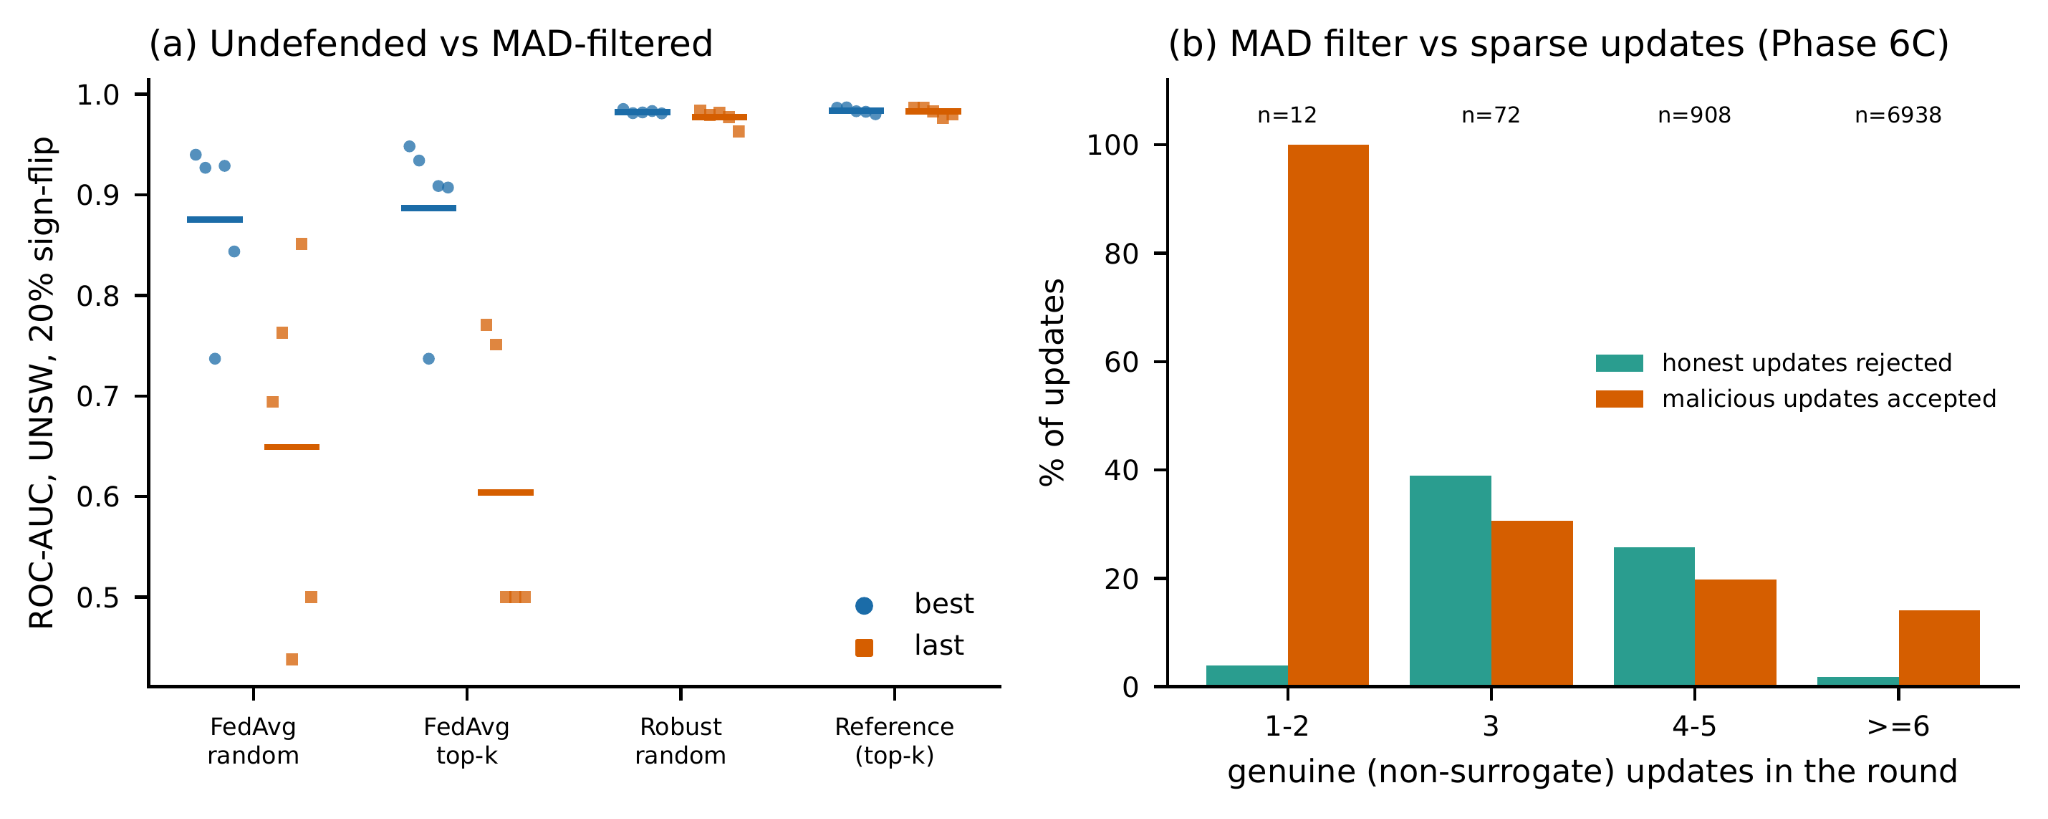
\includegraphics[width=\columnwidth]{fig2.png}
  \caption{Original UNSW-NB15 20\% sign-flip control:
  (a) selected-checkpoint versus last-round ROC--AUC;
  (b) MAD decisions by the number of genuine arrivals.}
  \label{fig:attack-robustness}
\end{figure}

\begin{figure*}[!t]
  \centering
  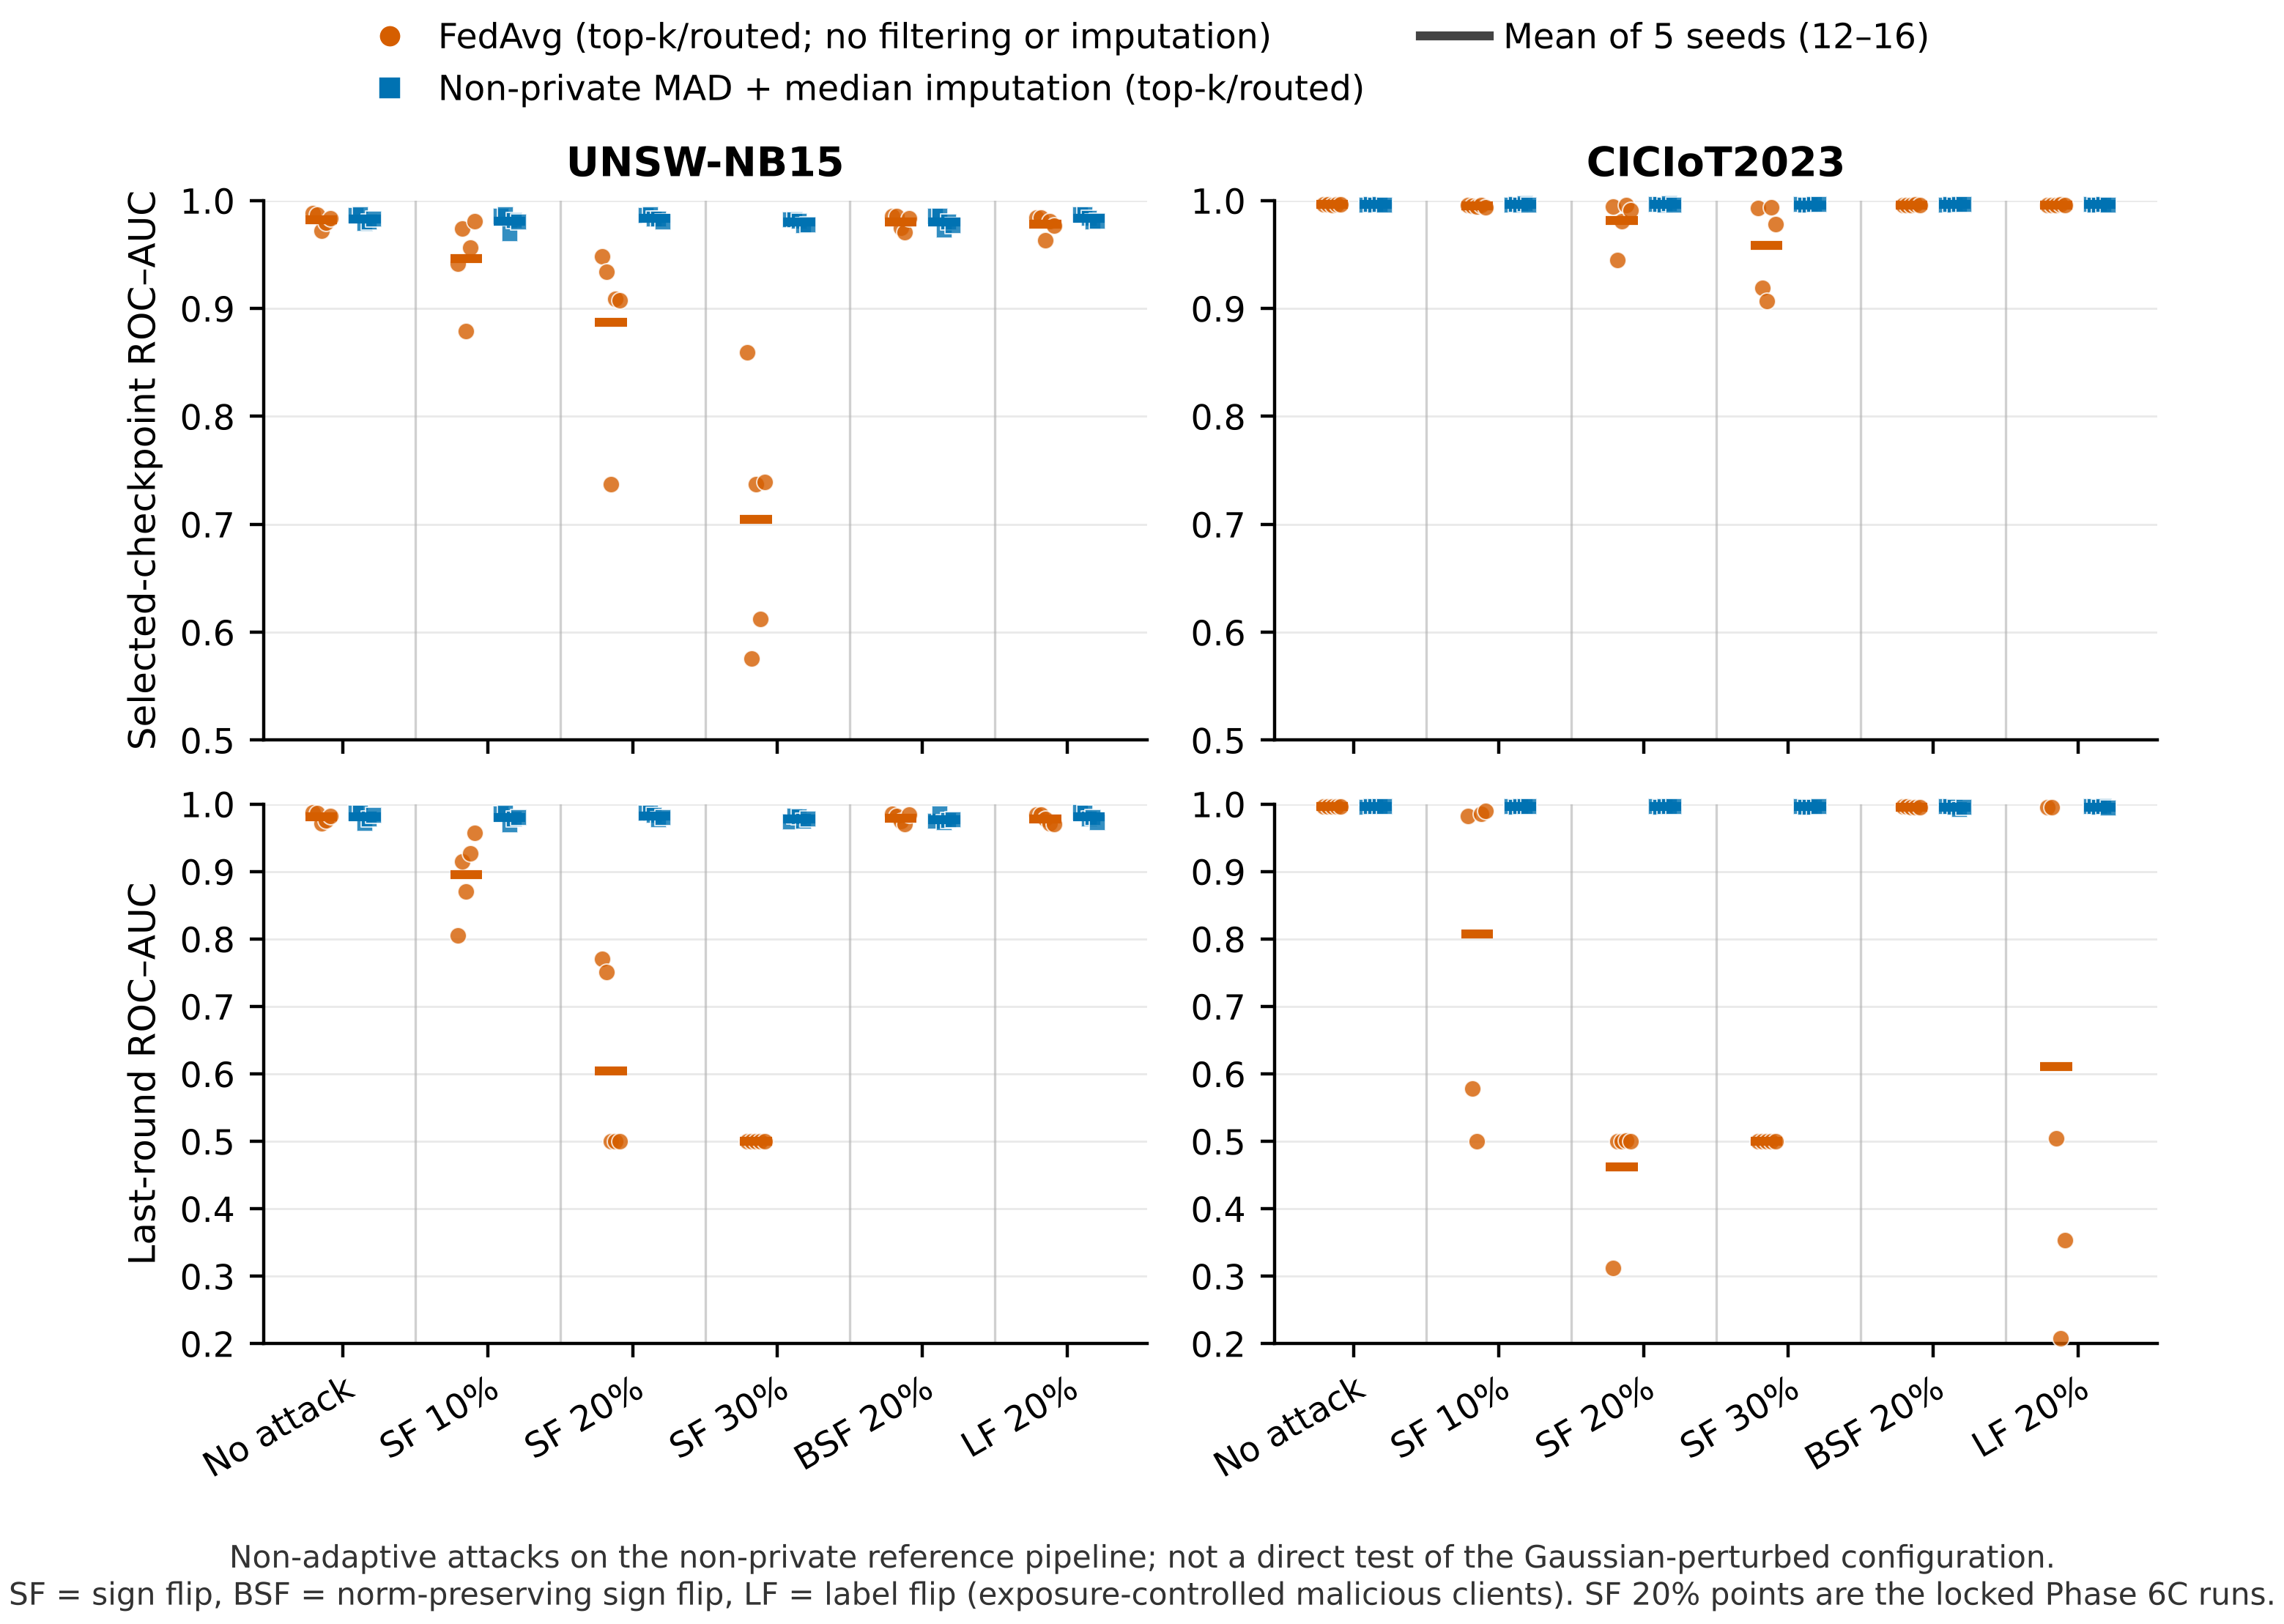
\includegraphics[width=0.93\textwidth]{fig3.png}
  \caption{Non-adaptive attack comparison using paired seeds 12--16
  	on UNSW-NB15 and CICIoT2023. Both arms use top-$k$ selection
  	and routed paths: orange circles, unfiltered FedAvg; blue squares,
  	non-private MAD with median imputation. Top/bottom panels show
  	selected/last-round ROC--AUC; markers indicate seeds and bars means.
  	SF: sign flip; BSF: norm-preserving sign flip; LF: label flip.
  	The Gaussian-perturbed configuration and adaptive attacks were not
  	evaluated.}
  \label{fig:attack-sweep}
\end{figure*}



\subsubsection{Controlled Detection and Network Performance}
\label{subsubsec:unsw-network}

Table~\ref{tab:overall-results} separates routing, selection and
aggregation controls on the locked validation/report partitions.
For CICIoT2023, changing FedAvg from uniform selection with random
paths (UR/X) to uniform selection with routed paths (UR/R)
reduced mean delivery delay from 87.3 to 71.8~ms and raised
first-transmission packet PDR from 0.694 to 0.782. Path stability
rose from 0.523 to 0.855. The corresponding UNSW-NB15 path
control reduced delay from 97.4 to 82.0~ms with the same PDR
and stability changes. These network outcomes do not isolate
a detection benefit, and delivered-update delay is not online
intrusion-alert latency.

The proposed $\widehat\varepsilon\approx20$ rows achieved F1 and
selected-checkpoint ROC--AUC of 0.9914/0.9937 (CICIoT2023)
and 0.9065/0.9522 (UNSW-NB15), respectively. Their routing
conditions are matched to FedAvg (top-$k$/routed) in Table~\ref{tab:overall-results};
therefore the identical mean network measurements cannot be
attributed to MAD filtering or Gaussian perturbation. Against
FedAvg with random paths and uniform selection, the comparison
changes several mechanisms at once.

Benign FPR remains approximately 0.1468 on CICIoT2023 and
0.1455 on UNSW-NB15, corresponding to about 147 and 146
false alarms per 1,000 benign validation/report records.
Because the classification threshold was calibrated under a
validation FPR cap of 0.15, these figures do not demonstrate an
acceptable deployment false-alarm burden.

\subsubsection{Routing and Surrogate Imputation: a Matched \texorpdfstring{$2\times2$}{2 x 2} Control}
\label{subsec:routing-surrogate}

Figure~\ref{fig:routing-surrogate} summarizes a non-private $2\times2$ control varying routing and
surrogate imputation using identical splits and five paired seeds.
On UNSW-NB15, selected-checkpoint AUC for routing on was
0.9822 without surrogates and 0.9838 with them; with routing
off, it was 0.9737 and 0.9685, respectively.
The interaction difference was +0.0068 (unadjusted 95\%
$t$-interval [$-0.0024$, +0.0159]); on CICIoT2023 it was
+0.0005 [$-0.0004$, +0.0014]. Neither interval establishes an
interaction or an independent detection benefit from surrogate
imputation. Reconstructed median vectors cannot recover the
missing clients' private training information.

\begin{figure*}[!t]
  \centering
  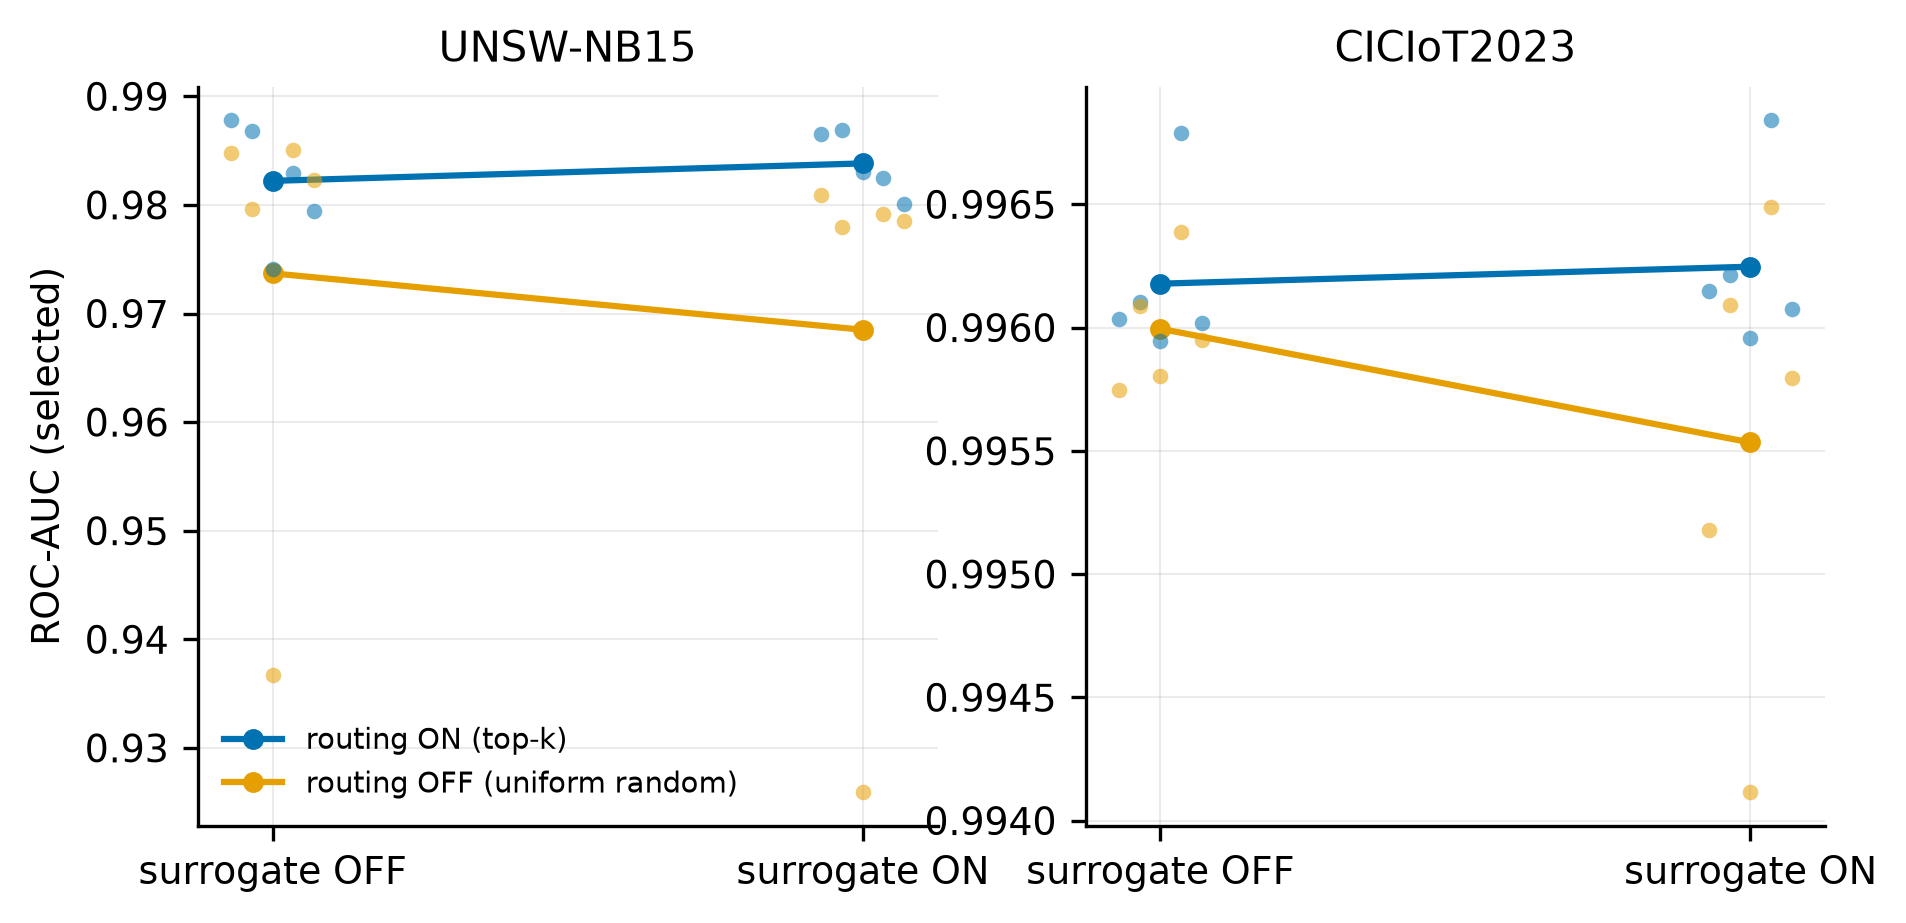
\includegraphics[width=0.87\textwidth]{fig4.png}
  \caption{Routing $\times$ surrogate-imputation control: selected
  ROC--AUC for five paired seeds under the four routing/imputation
  combinations. The two datasets are evaluated separately; the
  non-private controls do not establish an effect in the Gaussian
  pipeline. Shown comparisons are exploratory.}
  \label{fig:routing-surrogate}
\end{figure*}



\subsection{Participation Fairness and Held-out Client Recall}
\label{subsec:attack-routing-tradeoffs}

Top-$k$ routing preferentially selects well-connected clients; this
is a reliability objective rather than a fairness guarantee.
Figure~\ref{fig:participation-new} summarizes the matched
participation study. Across five seeds, selection Gini was
approximately 0.73 for top-$k$, 0.49 for coverage-aware
and 0.21 for uniform selection, while the average number of
never-selected clients was 27, 8 and 0 of 50, respectively.

Held-out client recall was measured only on evaluation rows that
were never used for training, with eligible clients requiring at
least ten held-out attack examples. UNSW-NB15 used the SUPP\_V1
holdout; CICIoT2023 used the SUPP\_V2 group-disjoint predictor
holdout fitted with training-only preprocessing. The two
protocols are therefore reported separately rather than pooled.
On UNSW-NB15 under independent network assignment, the mean
worst eligible-client recall was 0.916 for top-$k$ versus 0.779
for uniform selection. The mean paired difference was $-0.1375$
(unadjusted 95\% $t$-interval [$-0.260$,$-0.015$]); the two-sided
exact sign-flip test gave $p=0.0625$. With only five seeds and
many exploratory comparisons, this is not a confirmatory
superiority or harm claim. Greater participation coverage did
not consistently improve the least-served eligible client's recall.

\begin{figure*}[!t]
  \centering
  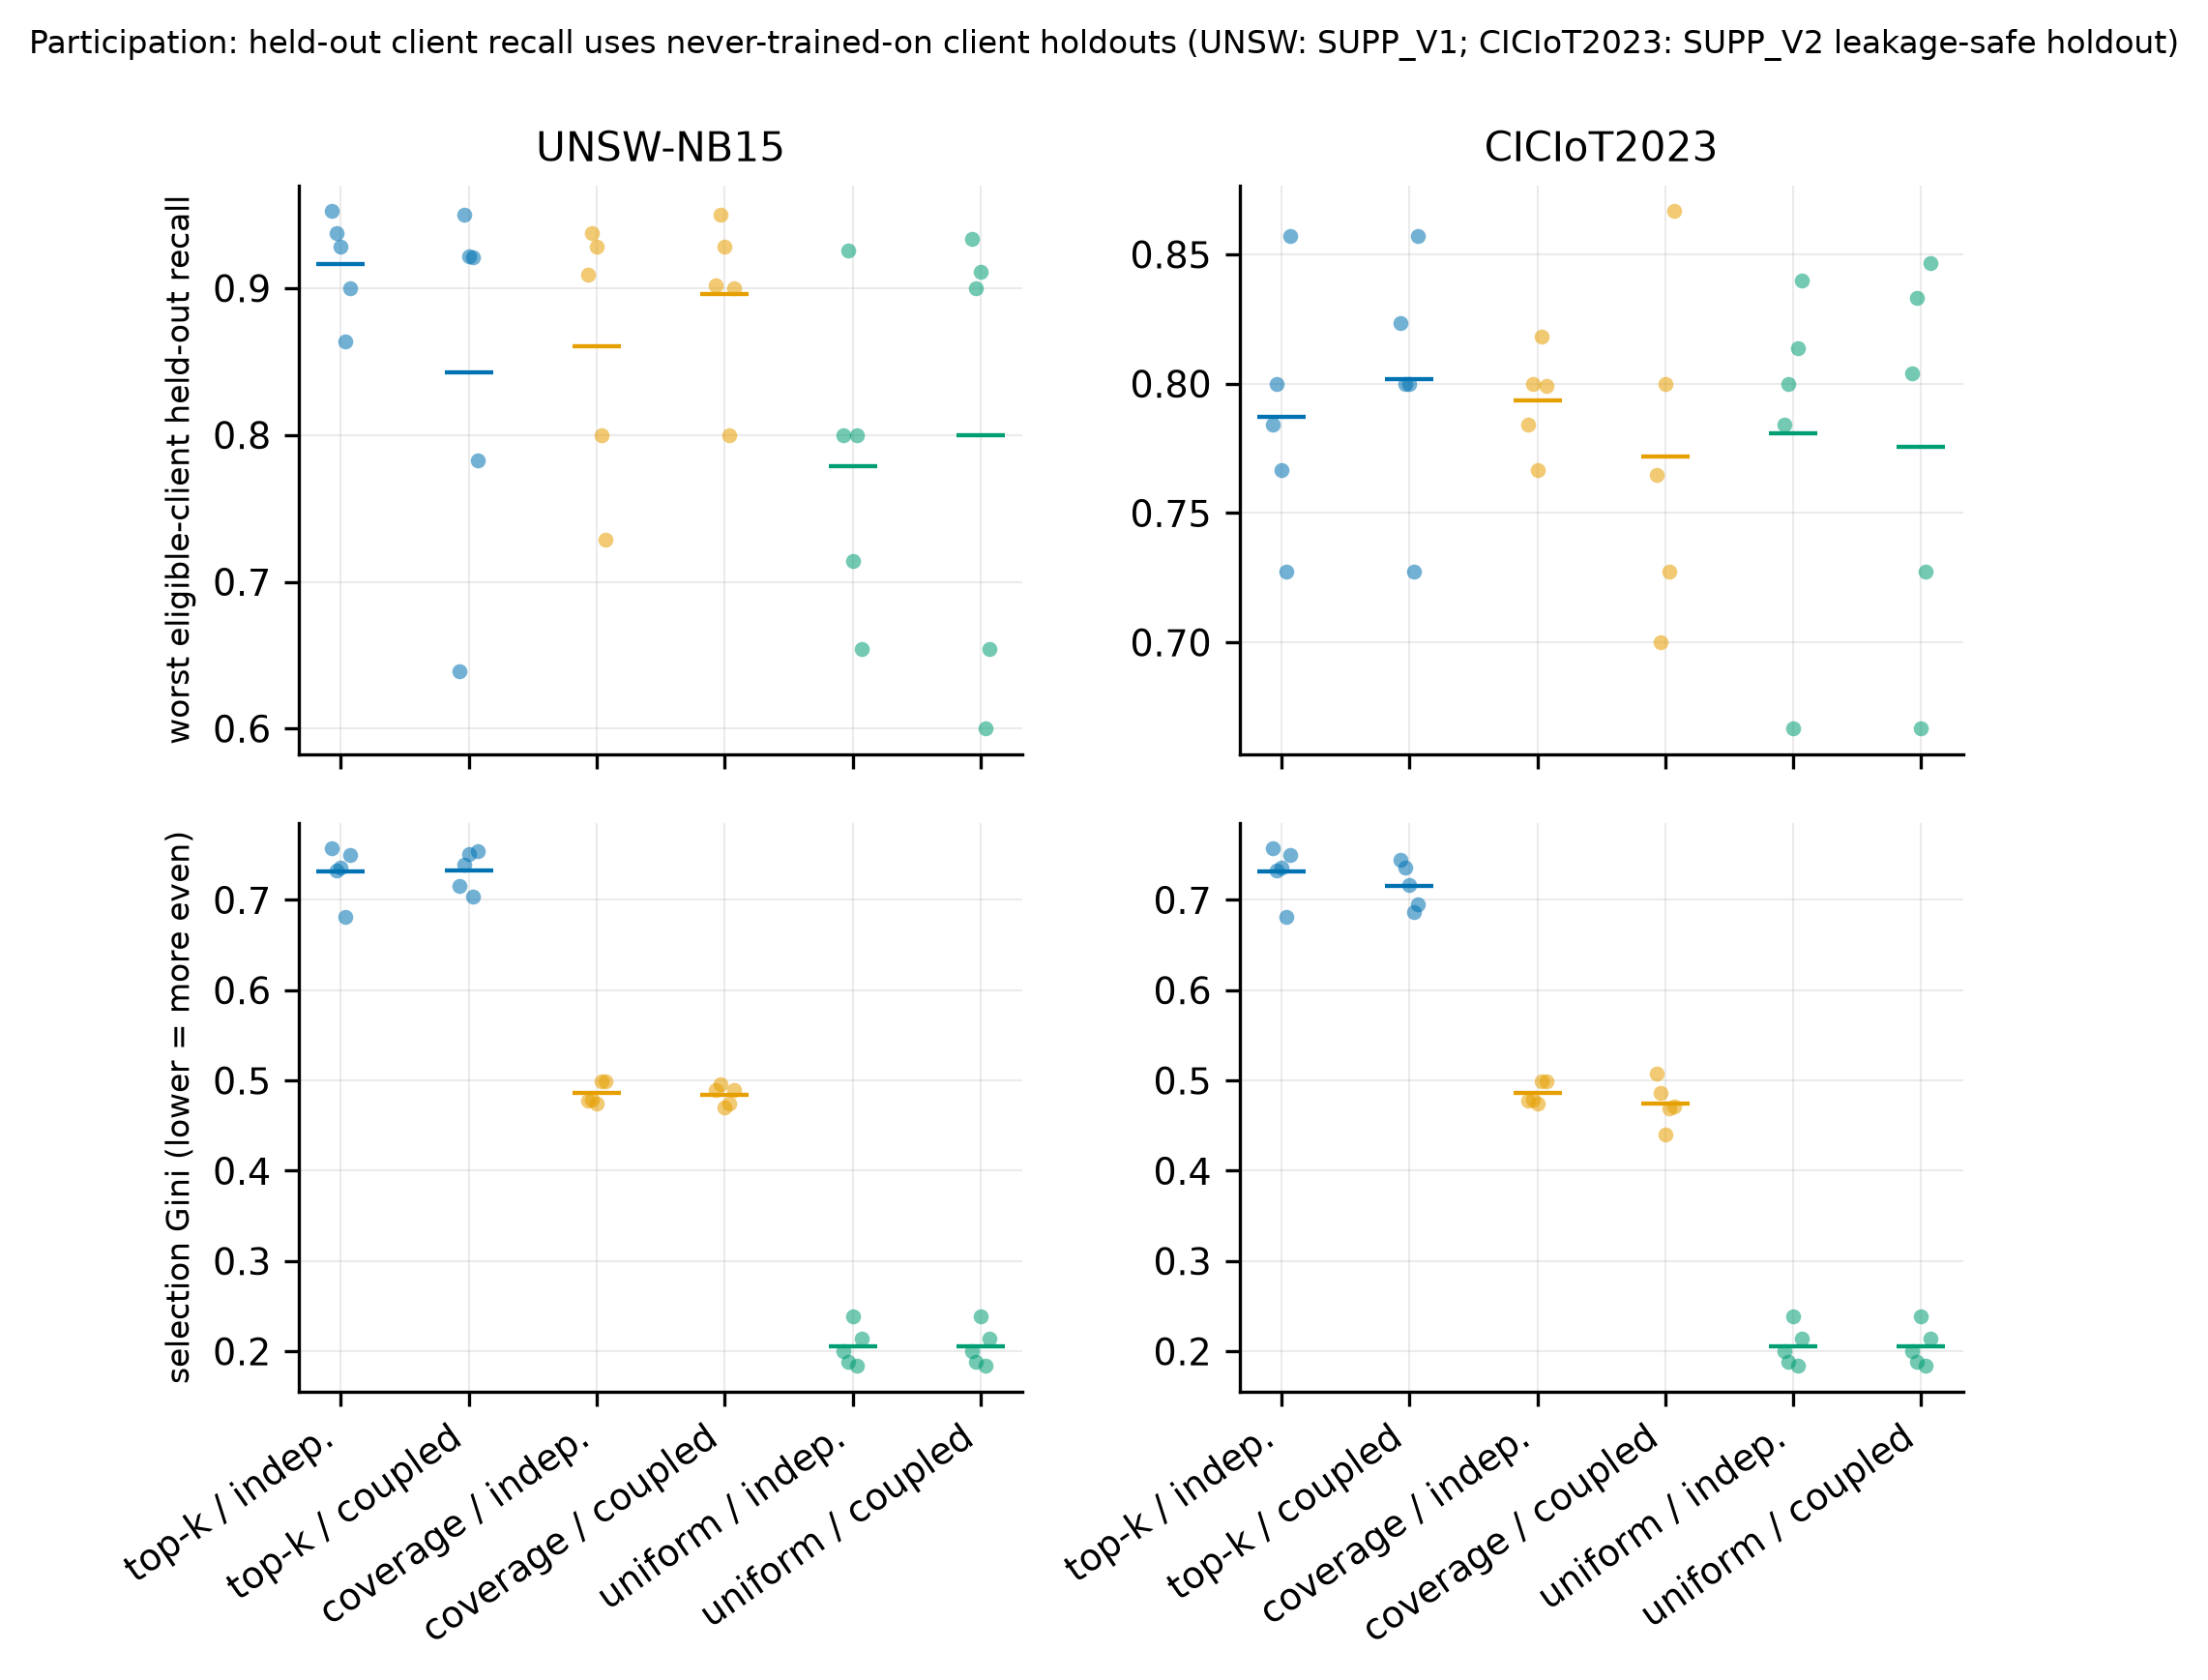
\includegraphics[width=0.85\textwidth]{fig5.png}
  \caption{Participation and client-level holdout outcomes: worst
  eligible-client attack recall (top) and selection Gini (bottom)
  for top-$k$, coverage-aware and uniform selection with independent
  and coupled simulated networks. Dots are five seeds, bars are
  means. UNSW-NB15 and CICIoT2023 use separate SUPP\_V1 and
  leakage-controlled SUPP\_V2 holdout protocols, respectively.}
  \label{fig:participation-new}
\end{figure*}



\subsection{Ablation}
\label{subsec:ablation}

We examined the contribution of the framework components on CICIoT2023
and UNSW-NB15 through paired comparisons using five random seeds
(12--16). The evidence comprises 130 audited historical runs and 40
current-code runs. The latter reproduced the reference configuration
and evaluated the robust-filtering and privacy-pipeline controls; the
other historical variants were verified against the evaluation ledger
rather than fully rerun. All reported ROC--AUC values in this section
refer to the validation/report partition, not the reserved test set.
We distinguish the selected validation checkpoint from the last
communication round (round 30). Differences are computed for matched
seeds as variant minus comparator. Single-factor controls are
interpreted separately from comparisons that change multiple stages.

\subsubsection{Effect of Robust Filtering on Training Stability}
\label{subsubsec:ablation-robust}

Removing median absolute deviation (MAD)-based filtering caused the
largest observed single-factor reduction in last-round ROC--AUC.
As shown in Figure~\ref{fig:ablation-robust}, the mean paired
selected-checkpoint differences were $-0.011$ on CICIoT2023 and
$-0.093$ on UNSW-NB15, with reported uncertainty intervals spanning
zero. In contrast, last-round differences reached $-0.309$ and
$-0.518$, respectively, and all five seeds showed lower final-round
ROC--AUC without robust filtering. The last-round ROC--AUC fell more
than 0.05 below the selected checkpoint for four of five unfiltered
CICIoT2023 runs and all five unfiltered UNSW-NB15 runs; this did not
occur in any matched reference run. Thus, checkpoint selection can
conceal substantial late-round instability when anomalous updates are
not filtered.

\begin{figure*}[!b]
	\centering
	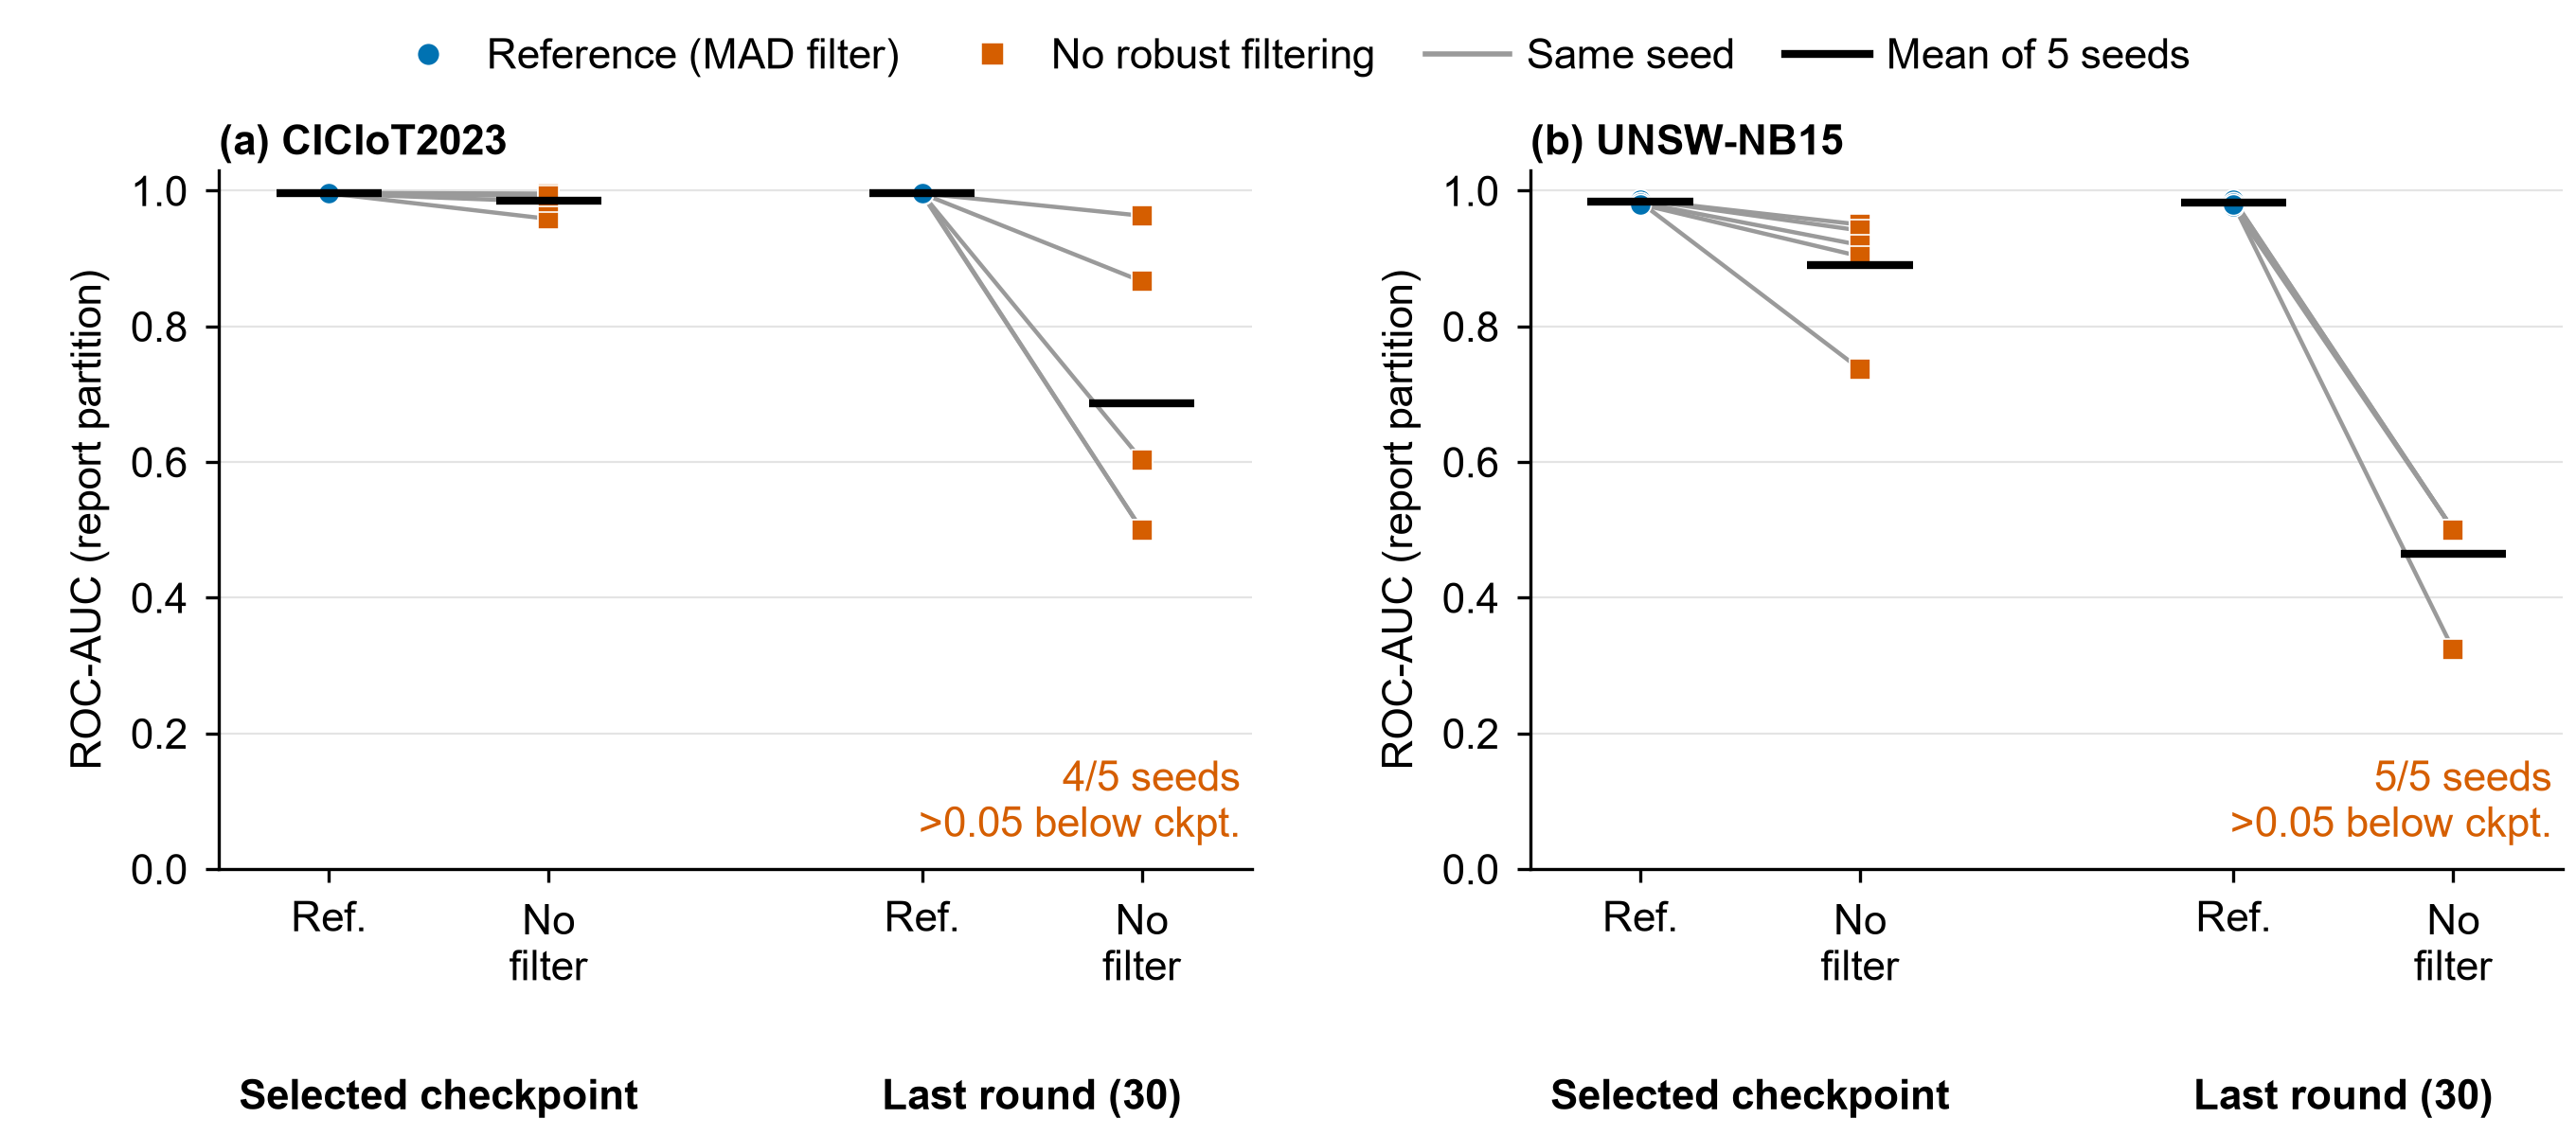
\includegraphics[width=0.94\textwidth]{fig6.png}
	\caption{Effect of disabling MAD-based robust filtering on
		validation/report-partition ROC--AUC: (a) CICIoT2023 and
		(b) UNSW-NB15. Each pair of markers represents the same random
		seed ($n=5$); horizontal black bars indicate five-seed means.
		Selected-checkpoint results are distinguished from round-30
		results.}
	\label{fig:ablation-robust}
\end{figure*}

\subsubsection{Other Components and Privacy-Pipeline Effects}
\label{subsubsec:ablation-components}

Figure~\ref{fig:ablation-components} compares paired ROC--AUC
changes for the remaining controls. Omitting surrogate imputation,
disabling server momentum while holding the server learning rate at
$\eta_s=0.5$, and applying MAD filtering to genuine updates before
surrogate reconstruction did not produce clearly distinguishable
selected-checkpoint effects across the five seeds. This is not
evidence of equivalence. Client-selection policies likewise showed
small and variable detection differences, although participation
became more balanced: the selection Gini coefficient changed from
approximately 0.73 for top-$k$ selection to 0.49 for coverage-aware
selection and 0.21 for uniform selection; the mean numbers of
never-selected clients were 27.2, 8, and 0, respectively.

\begin{figure*}[!t]
	\centering
	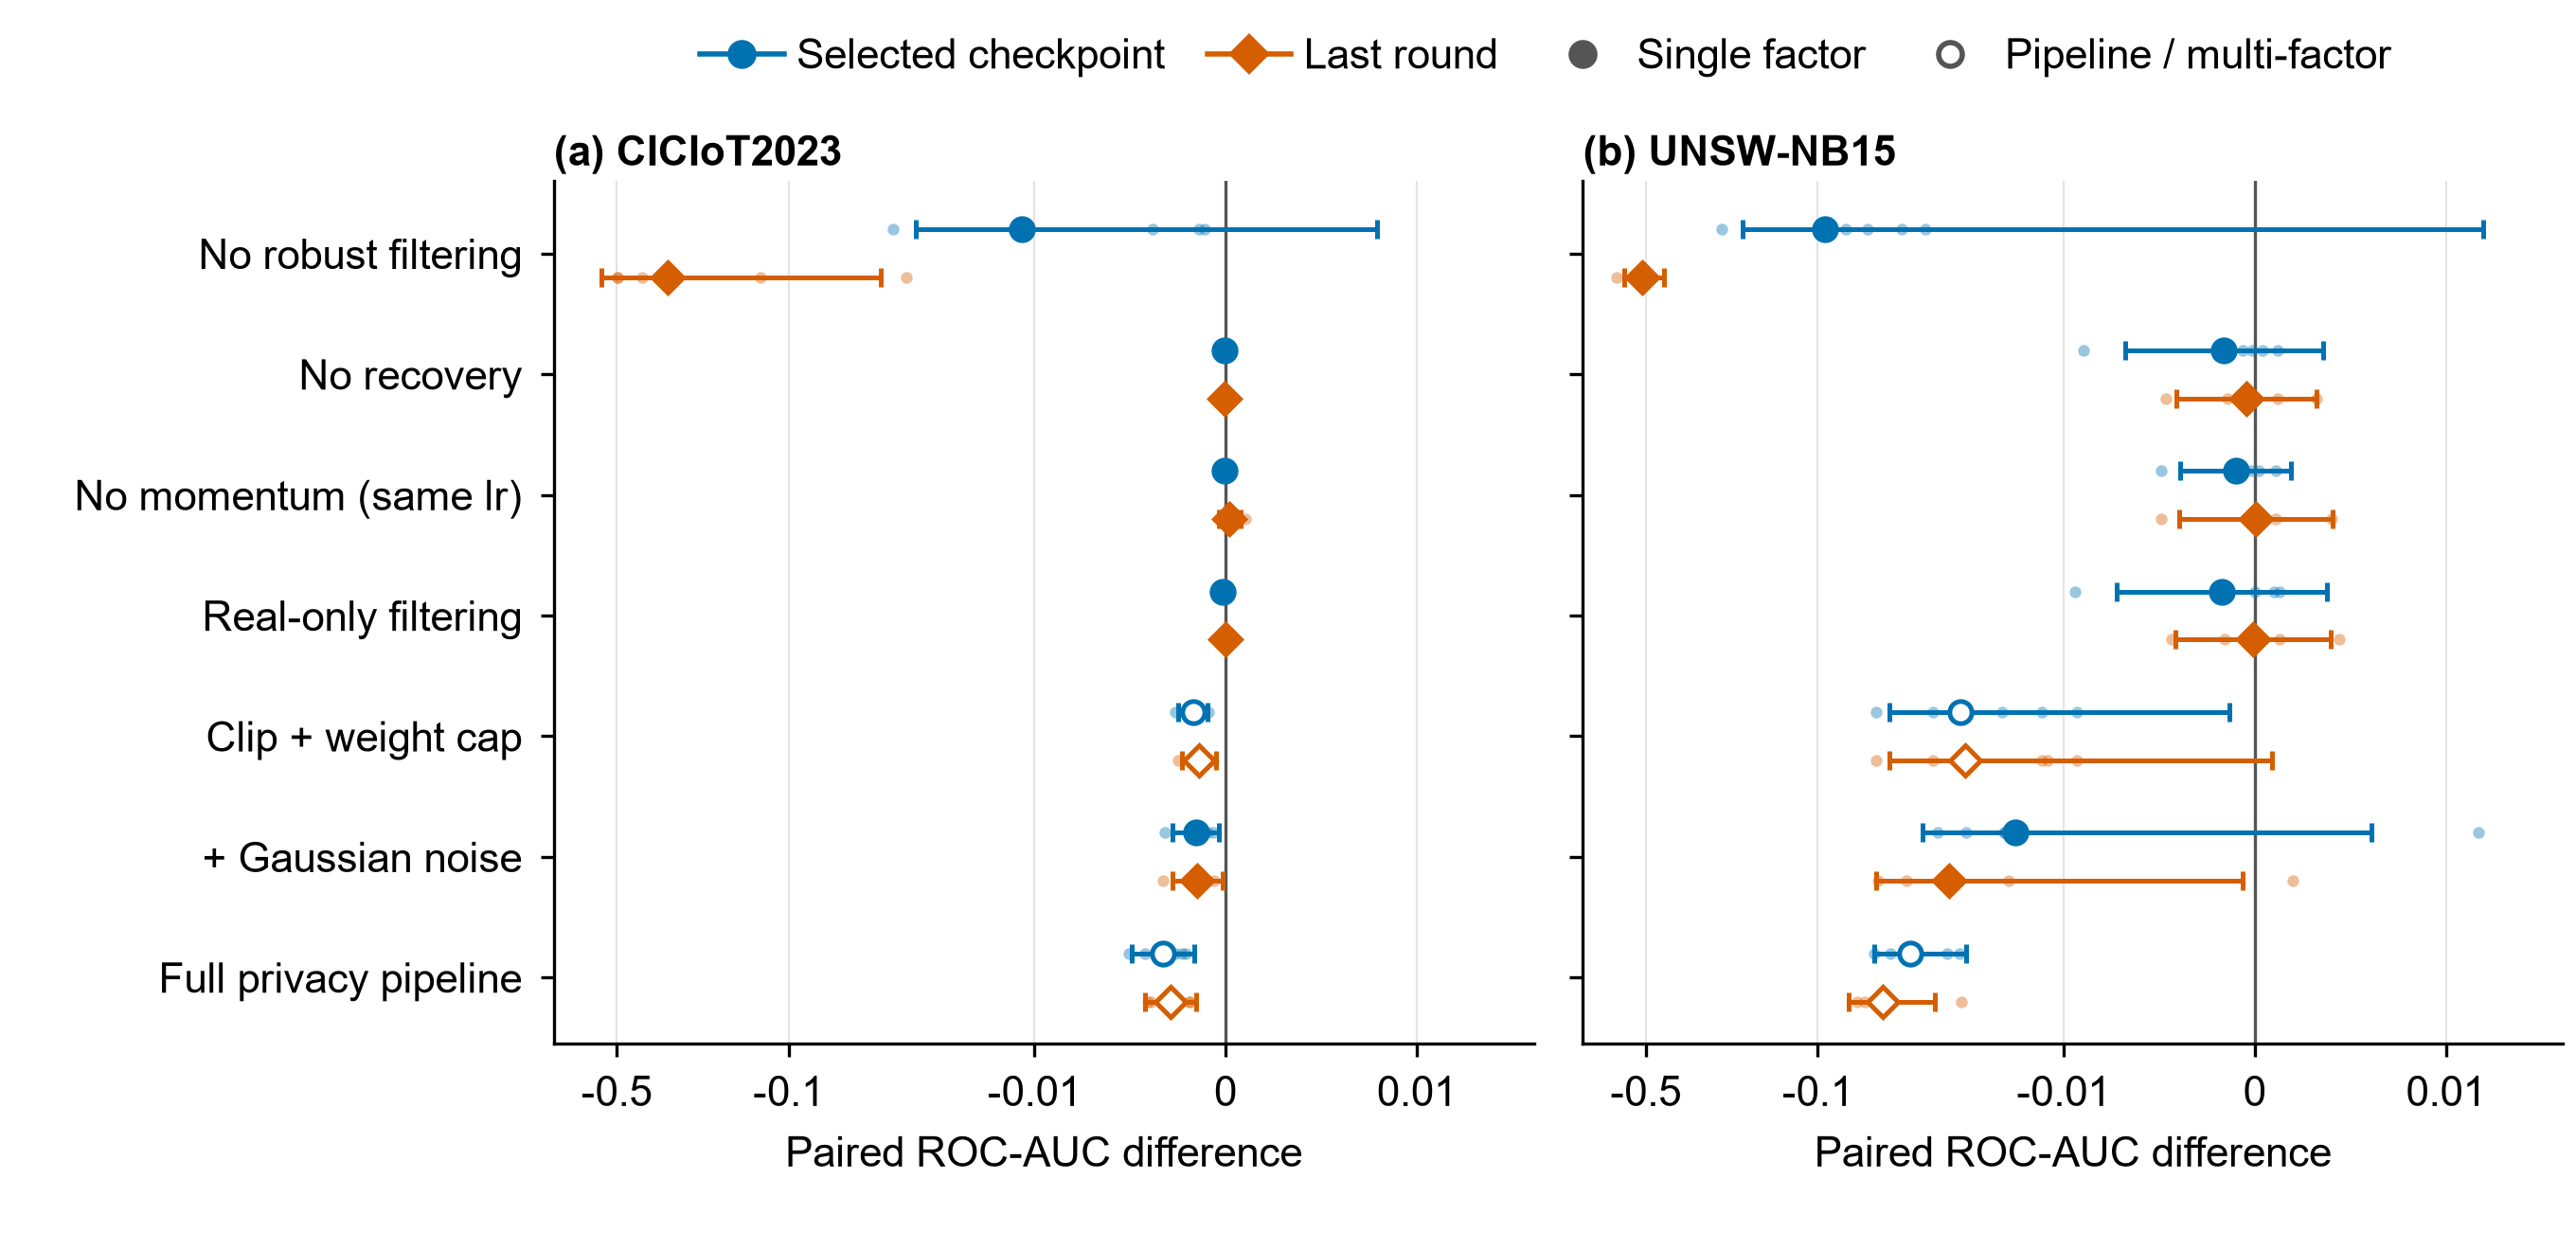
\includegraphics[width=0.94\textwidth]{fig7.png}
	\caption{Paired ROC--AUC changes (variant minus matched comparator)
		for CICIoT2023 and UNSW-NB15. Blue circles denote selected
		checkpoints and orange diamonds denote the last round; filled
		and hollow markers distinguish single-factor and pipeline-level
		contrasts. Horizontal intervals summarize uncertainty across
		paired seeds. The horizontal axis uses a symmetric-logarithmic
scale and privacy contrasts have different matched comparators.
The plotted ``Clip + weight cap'' category is a combined change in
clipping, aggregation path and heterogeneous-to-uniform weights,
not a cap-only effect.}
	\label{fig:ablation-components}
\end{figure*}

\begin{table}[!tbp]
	\caption{Audited mean paired ROC--AUC differences over five seeds
		(exploratory). The Gaussian-only row changes only noise under
		identical clipping, uniform weights and network traces; the other
		privacy rows combine a change to clipping, aggregation path and
		heterogeneous-to-uniform weighting.}
	\label{tab:ablation-summary}
	\centering
	\footnotesize
	\setlength{\tabcolsep}{3pt}
	\renewcommand{\arraystretch}{1.02}
	\begin{tabular}{@{}lrr@{}}
		\toprule
		Contrast (evaluation point) & CICIoT2023 & UNSW-NB15 \\
		\midrule
		No MAD filter (selected) & $-0.011$ & $-0.093$ \\
		No MAD filter (last) & $-0.309$ & $-0.518$ \\
		Clip + uniform (combined) & $-0.0017$ & $-0.0262$ \\
		Added Gaussian (noise only) & $-0.0015$ & $-0.0157$ \\
		Full pipeline (combined) & $-0.0032$ & $-0.0419$ \\
		\bottomrule
	\end{tabular}
\end{table}

Table~\ref{tab:ablation-summary} gives ordered contrasts, not
individual contributions from every component. The no-noise
``Clip + uniform'' comparison changes both clipping and the
aggregation mode, replacing heterogeneous sample-size weights
with uniform capped weights. Its paired AUC differences are
$-0.0017$ and $-0.0262$ on CICIoT2023 and UNSW-NB15.
Adding Gaussian noise to that already clipped, uniformly weighted
pipeline is a controlled \emph{noise-only} change ($-0.0015$
and $-0.0157$, respectively), because the clipping outcomes,
applied weights and selected network traces match by seed.
The full combined contrasts are $-0.0032$ and $-0.0419$.
The non-noise combined step represents approximately 53\% and
63\% of the respective point-estimate losses, but this is
\emph{not} a decomposition of clipping and weighting effects.
These five-seed comparisons are exploratory and the reported
$\widehat\varepsilon\approx10$ is diagnostic rather than a
certified privacy guarantee.



Communication changes require similar care. On CICIoT2023,
packet-coupled delivery reduced the delivered-update ratio from
approximately 0.848 to 0.681, increased delay from roughly
66--77~ms to 250--263~ms, and reduced genuine retained updates
from about 5.9 to 4.3 per round. Because this configuration changes
the delivery process, it is not an isolated ablation of the routing
algorithm. Likewise, a historical configuration combining zero
momentum with server learning rate 5.0 cannot identify the effect
of momentum alone. With only five paired seeds, a two-sided exact
sign-flip test has a minimum attainable $p$-value of 0.0625,
whereas parametric $t$-intervals can exclude zero. Such intervals
are unadjusted for the large number of exploratory comparisons
and do not establish definitive component effects. The
reported comparisons use audited metrics and exclude unregistered
checkpoint files.

\subsection{Parameter Sensitivity and Simulated Resource Scaling}
\label{subsec:sensitivity-scaling}

Parameter sweeps used matched seeds and the validation/report
protocol, not the reserved test sets. On UNSW-NB15 ($n=5$),
Dirichlet $\alpha=0.1$ relative to 0.5 decreased selected AUC by
$-0.1159$; its unadjusted 95\% interval ranged from $-0.2114$ to
$-0.0203$. Halving the clipping norm changed AUC by $-0.0187$
(interval $-0.0359$ to $-0.0015$). Other parameter effects
were small or imprecise. CICIoT2023 sensitivity runs used three
seeds for most parameters, so their uncertainty is less resolved.
Detailed confidence intervals appear in Supplementary Figure~S2. The $\chi_{\mathrm{rec}}$ sweep on the non-private reference is
kept distinct from the Gaussian-path $\chi_{\mathrm{rec}}=0$
abstention control (Table S6).



Figure~\ref{fig:scalability-new} summarizes a separate three-seed scalability study varying the total number
of simulated clients $N\in\{25,50,100\}$ and the selected count
$k\in\{5,10,20\}$. At $N=50$, $k=10$, selected AUC was about
0.9521 (UNSW-NB15) and 0.9929 (CICIoT2023); doubling $N$
while retaining $k=10$ yielded 0.9205 and 0.9908, respectively.
The simulated serialized-update traffic scales with $k$, from
26.2 to 104.7 MB per run on UNSW-NB15 and from 14.3 to
57.2 MB on CICIoT2023 when $k$ rises from 5 to 20.
Peak working-set measurements were approximately 1.03 GB and
2.56 GB, respectively, dominated by in-memory data. Wall times
were measured on one shared CPU host and must not be interpreted
as production IoT latency or a hardware scalability guarantee.

\begin{figure*}[!t]
  \centering
  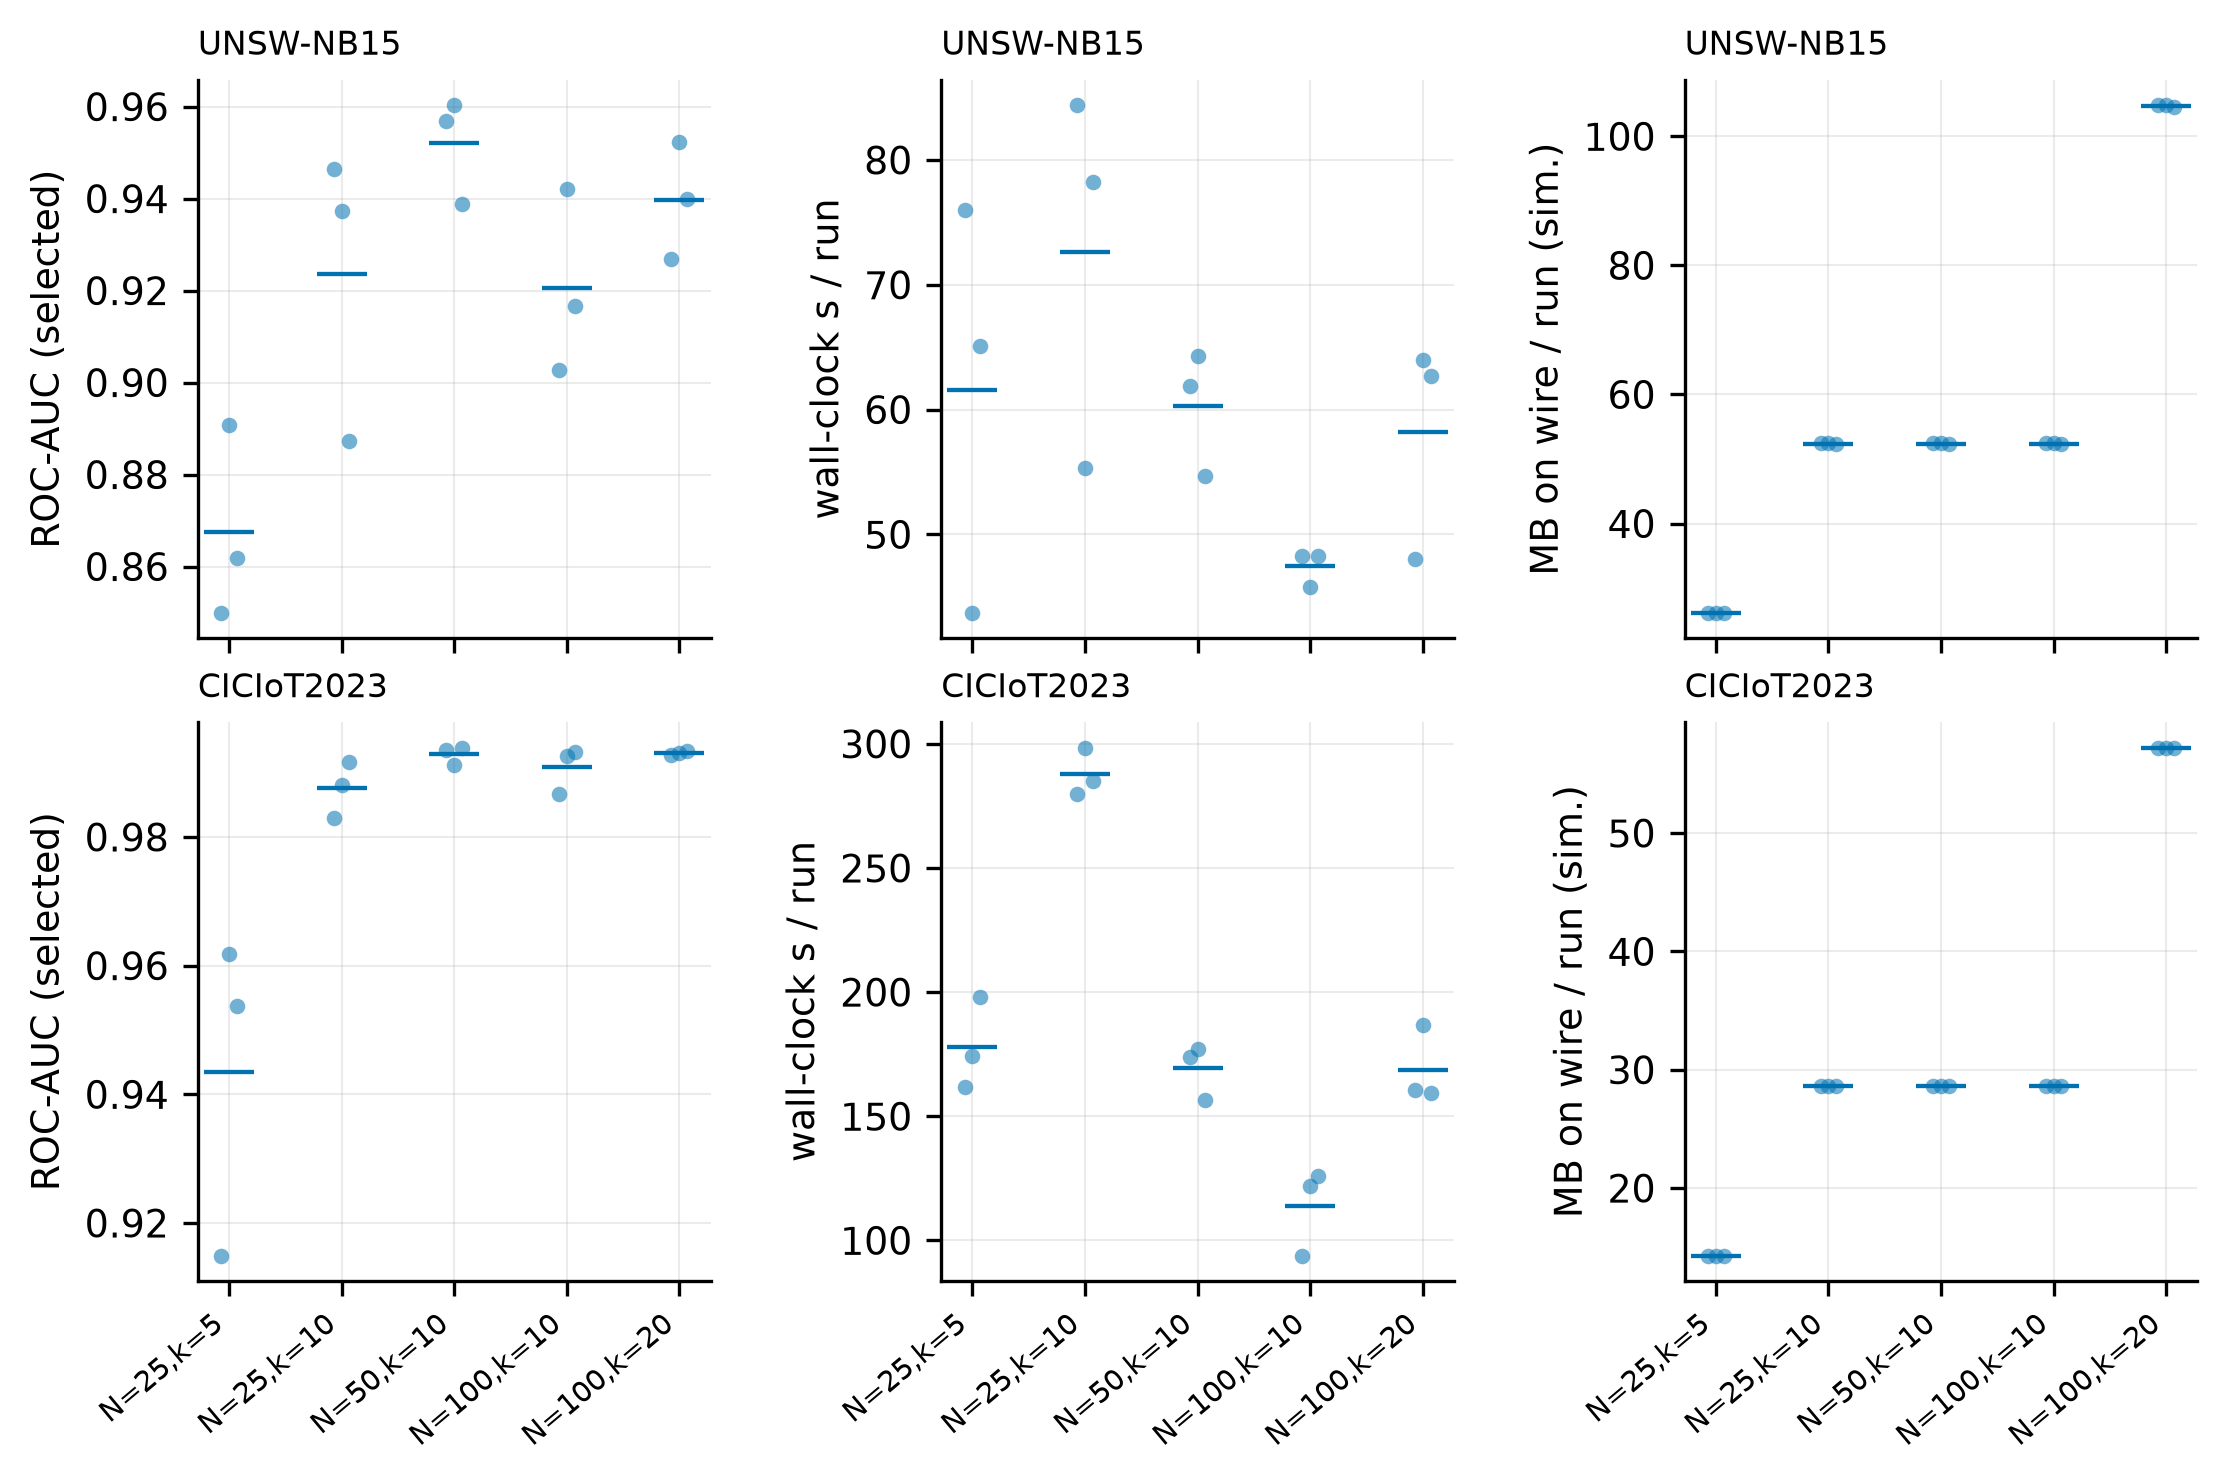
\includegraphics[width=0.93\textwidth]{fig8.png}
  \caption{Exploratory three-seed scalability controls for
  UNSW-NB15 (top) and CICIoT2023 (bottom): selected ROC--AUC,
  shared-host runtime, and simulated bytes on the wire for
  different $N$ and $k$. The network quantities are simulated and
  wall-clock values are not deployment benchmarks.}
  \label{fig:scalability-new}
\end{figure*}

\subsection{Controlled Failure Sensitivity and Privacy Diagnostics}
\label{subsec:resilience-privacy}

The audited reference configuration was examined under
explicit client-failure probabilities of 0, 0.1, and 0.3
on UNSW-NB15, using five random seeds. These experiments
represent a reference-configuration sensitivity analysis,
not an isolated evaluation of the full privacy-enabled
pipeline. Injected client failures occur in addition to
baseline network non-delivery; therefore, a zero injected
failure probability does not imply a failure-free network.

\subsubsection{Failure Sensitivity}
\label{subsubsec:failure-resilience}

Table~\ref{tab:failure-sensitivity} summarizes the observed
failure behavior. Mean failed clients per round increased
from 1.52 to 4.11 across the evaluated settings, while
the validation-F1 recovery fraction remained between
0.962 and 0.973.

\begin{table}[!tbp]
	\caption{Audited failure sensitivity of the UNSW-NB15
		reference configuration (five-seed means).}
	\label{tab:failure-sensitivity}
	\centering
	\footnotesize
	\setlength{\tabcolsep}{4pt}
	\begin{tabular}{@{}lccc@{}}
		\toprule
		$p_f$ &
		\shortstack{Failures\\per round} &
		\shortstack{F1 recovery\\fraction} &
		\shortstack{Recovery\\rounds} \\
		\midrule
		0.0 & 1.52 & 0.962 & 1.12 \\
		0.1 & 2.50 & 0.963 & 1.11 \\
		0.3 & 4.11 & 0.973 & 1.20 \\
		\bottomrule
	\end{tabular}
\end{table}

The reported recovery fraction measures the proportion
of failure events followed by restoration of smoothed
validation F1-score to at least 95\% of its pre-failure
value. It is distinct from surrogate-imputation coverage.
F1 recovery did not decline monotonically as injected
failures increased.

The observed packet delivery ratio and mean delay
remained approximately 0.8511 and 76.65~ms across
all three settings. Since explicit client failures did
not modify the network-delivery process, these constant
network metrics do not establish an independent
failure-mitigation effect of routing-aware selection.

\subsubsection{Privacy Diagnostics}
\label{subsubsec:privacy-cost}

For the audited Gaussian reference configuration, the
estimated privacy-accounting budget was approximately
$\widehat{\varepsilon}=9.999$. The corresponding
noise-to-signal ratios were approximately 23.53 on
CICIoT2023 and 35.29 on UNSW-NB15.


The new Table~\ref{tab:overall-results} also reports completed
DP+FedAvg and $\varepsilon\approx20$ controls. Comparisons across
these configurations are multi-factor and should not be used to
attribute utility effects solely to Gaussian noise. Moreover,
deterministic client selection and data-dependent
filtering are not fully represented by the accounting
approximation. Thus, the reported privacy budget is
not a certified end-to-end differential-privacy
guarantee.

The ablation results in Section~\ref{subsec:ablation} isolate
an incremental Gaussian-only utility change, but the other
contrasts combine clipping and the transition from heterogeneous
to uniform weights. Their separate effects were not identified.
Consequently, privacy-related utility differences must be
interpreted at the specified pipeline level.


\section{Conclusion}
\label{sec:conclusion}

This study evaluated routing-aware update delivery with
median-based surrogate imputation, MAD filtering and optional
Gaussian-perturbed aggregation for federated IDS training under
simulated Edge--Cloud communication failures. On the locked
validation/report partitions, the $\widehat\varepsilon\approx20$
configuration achieved F1/ROC--AUC of 0.9914/0.9937 on CICIoT2023
and 0.9065/0.9522 on UNSW-NB15. Against random-path,
uniform-selection FedAvg, CICIoT2023 simulated update delay
changed from 87.3 to 66.0~ms and first-transmission PDR from
0.694 to 0.851, but this is a multi-component comparison.

Under a static 30\% sign-flip attack, the non-private MAD-plus-
surrogate reference retained a selected-checkpoint AUC of 0.9799
on UNSW-NB15 versus 0.7046 for unfiltered FedAvg. This contrast
supports conditional robustness to the tested sign-flip model,
not a guarantee against adaptive attacks. The matched routing
$\times$ imputation controls found no demonstrated standalone
detection benefit from inserting median surrogates. In the
central-Gaussian pipeline, the weight cap forces exactly uniform
weights with at most ten retained updates; neither client sample
size nor $\chi_{\mathrm{rec}}$ influences the applied weights in
those non-abstaining rounds. The utility loss attributed to the
non-noise privacy step combines clipping and reweighting,
whereas the incremental Gaussian-noise contrast is isolated.

Selection policies with lower participation concentration did
not consistently improve the worst eligible-client held-out
recall. Resource and sensitivity measurements come from small
paired-seed simulations and shared-host CPU runs. Benign FPR
near 0.15, incomplete capture-level independence in parts of
CICIoT2023, untested adaptive poisoning, and the absence of a
real Edge--Cloud testbed constrain deployment conclusions.
Finally, individual updates are visible to the receiving server
and the RDP estimates rely on a sampling approximation that does
not certify privacy under deterministic selection and filtering.
Future work should address adaptive attackers, stronger
independent-data evaluation, operational false-alarm thresholds,
and a privacy mechanism with an appropriate formal accountant.



	\section*{Code Availability}

The implementation, locked configurations and analysis scripts are
available in the \href{https://github.com/RezaAzarnia/routing-aware-fl-edgecloud-iot-ids}{GitHub repository}.
The versioned \href{https://doi.org/10.5281/zenodo.24032087}{Zenodo snapshot}
(\texttt{v.1.0.5}, commit \texttt{7d598855}) predates SUPP\_V1/V2 and
does not archive their new attack, sensitivity, participation or
scalability results.

\section*{Data Availability}

\href{https://cicresearch.ca/IOTDataset/CIC_IOT_Dataset2023/}{CICIoT2023}
and \href{https://www.kaggle.com/datasets/mrwellsdavid/unsw-nb15}{UNSW-NB15}
are publicly available; their raw datasets are not redistributed.
The \href{https://doi.org/10.5281/zenodo.24032087}{v.1.0.5 archive}
includes the controlled Table~\ref{tab:overall-results} manifest and
per-seed, summary and paired-effect CSVs (seeds 12--16).
New SUPP\_V1/V2 per-seed, summary, figure-data and QA files are supplied
separately with this revision, not in that archive. Complete raw
run outputs, checkpoints and validation predictions are not publicly archived.

\FloatBarrier
	\setlength{\bibsep}{0pt}
\interlinepenalty=10000
	\bibliographystyle{elsarticle-num}
	\bibliography{references}
	
\end{document}
